\documentclass[compress]{beamer}
\mode<presentation>
\setbeamercovered{transparent}
\usetheme{Warsaw}
%\useoutertheme{smoothtree}
\usepackage{multirow}
\usepackage[english]{babel}
\usepackage[latin1]{inputenc}
\usepackage{times}
\usepackage[T1]{fontenc}
\usepackage{xmpmulti}
\usepackage{multicol}
\usepackage{colortbl}



%\setbeamersize{text margin left=.25 in,text margin right=.25 in}
\setbeamersize{text margin left=.15 in,text margin right=.15 in}
\usepackage[authoryear]{natbib}


\usepackage{epstopdf}
\usepackage{xcolor}
\usepackage{latexcolors}
%\usepackage[dvipsnames]{xcolor}
\definecolor{antiquebrass}{rgb}{0.8, 0.58, 0.46}
\definecolor{babyblueeyes}{rgb}{0.63, 0.79, 0.95}
\definecolor{babyblue}{rgb}{0.54, 0.81, 0.94}
\definecolor{bistre}{rgb}{0.24, 0.17, 0.12}
\definecolor{brightlavender}{rgb}{0.75, 0.58, 0.89}
\definecolor{bulgarianrose}{rgb}{0.28, 0.02, 0.03}
\definecolor{slateblue}{rgb}{0.56, 0.74, 0.56}
\definecolor{cordovan}{rgb}{0.54, 0.25, 0.27}
\definecolor{darkbyzantium}{rgb}{0.36, 0.22, 0.33}

\setbeamercolor{structure}{fg=bittersweet!90, bg= black!60}







\usepackage{tikz}
\usetikzlibrary{shadows,calc}
\usetikzlibrary{shadows.blur}
\usetikzlibrary{shapes.symbols}
\usepackage{hyperref}
\usepackage{booktabs}
\usepackage{colortbl}
\usepackage{multirow}
%%%%%%%%% shaddow image %%%%%
% some parameters for customization
\def\shadowshift{3pt,-3pt}
\def\shadowradius{6pt}
\colorlet{innercolor}{black!60}
\colorlet{outercolor}{gray!05}
% this draws a shadow under a rectangle node
\newcommand\drawshadow[1]{
\begin{pgfonlayer}{shadow}
    \shade[outercolor,inner color=innercolor,outer color=outercolor] ($(#1.south west)+(\shadowshift)+(\shadowradius/2,\shadowradius/2)$) circle (\shadowradius);
    \shade[outercolor,inner color=innercolor,outer color=outercolor] ($(#1.north west)+(\shadowshift)+(\shadowradius/2,-\shadowradius/2)$) circle (\shadowradius);
    \shade[outercolor,inner color=innercolor,outer color=outercolor] ($(#1.south east)+(\shadowshift)+(-\shadowradius/2,\shadowradius/2)$) circle (\shadowradius);
    \shade[outercolor,inner color=innercolor,outer color=outercolor] ($(#1.north east)+(\shadowshift)+(-\shadowradius/2,-\shadowradius/2)$) circle (\shadowradius);
    \shade[top color=innercolor,bottom color=outercolor] ($(#1.south west)+(\shadowshift)+(\shadowradius/2,-\shadowradius/2)$) rectangle ($(#1.south east)+(\shadowshift)+(-\shadowradius/2,\shadowradius/2)$);
    \shade[left color=innercolor,right color=outercolor] ($(#1.south east)+(\shadowshift)+(-\shadowradius/2,\shadowradius/2)$) rectangle ($(#1.north east)+(\shadowshift)+(\shadowradius/2,-\shadowradius/2)$);
    \shade[bottom color=innercolor,top color=outercolor] ($(#1.north west)+(\shadowshift)+(\shadowradius/2,-\shadowradius/2)$) rectangle ($(#1.north east)+(\shadowshift)+(-\shadowradius/2,\shadowradius/2)$);
    \shade[outercolor,right color=innercolor,left color=outercolor] ($(#1.south west)+(\shadowshift)+(-\shadowradius/2,\shadowradius/2)$) rectangle ($(#1.north west)+(\shadowshift)+(\shadowradius/2,-\shadowradius/2)$);
    \shade[outercolor,right color=innercolor,left color=innercolor] ($(#1.north west)+(-\shadowradius/12,\shadowradius/12)$) rectangle ($(#1.south east)+(\shadowradius/12,-\shadowradius/12)$);%Frame
    \filldraw ($(#1.south west)+(\shadowshift)+(\shadowradius/2,\shadowradius/2)$) rectangle ($(#1.north east)+(\shadowshift)-(\shadowradius/2,\shadowradius/2)$);
\end{pgfonlayer}
}
% create a shadow layer, so that we don't need to worry about overdrawing other things
\pgfdeclarelayer{shadow} 
\pgfsetlayers{shadow,main}
% Define image shadow command
\newcommand\shadowimage[2][]{%
\begin{tikzpicture}
\node[anchor=south west,inner sep=0] (image) at (0,0) {\includegraphics[#1]{#2}};
\drawshadow{image}
\end{tikzpicture}}
\usepackage{calligra}

\DeclareMathOperator*{\argmax}{Arg\,max}
\DeclareMathOperator*{\argmin}{Arg\,min}
\newcommand{\norm}[1]{\left\Vert #1 \right\Vert }
\newcommand{\bbetaHat}{ \widehat{\bbeta}}
\newcommand{\bbetaLSE}{ \widehat{\bbeta}_{_{\text{LSE}}}}
\newcommand{\bbetaMLE}{ \widehat{\bbeta}_{_{\text{MLE}}}}
\newcommand{\sqBullet}[1]{  {\tiny \tiny \tiny \qBoxCol{#1!60}{ }} }
%***************
%\newtheorem{thm}{Theorem}
%\documentclass[noinfoline]{imsart}
%\usepackage{amsmath,amstext,amssymb}
%%\usepackage[top=1.5in, bottom=1.5in, left=1.2in, right=1.2in]{geometry}
%% settings
%%\pubyear{2005}
%%\volume{0}
%%\issue{0}
%%\firstpage{1}
%%\lastpage{8}
%\arxiv{arXiv:0000.0000}

%\startlocaldefs
%\numberwithin{equation}{section}
%\theoremstyle{plain}
%\newtheorem{thm}{Theorem}
%\endlocaldefs
\usepackage{lipsum} 
\usepackage{amsmath}
\usepackage{amssymb}
\usepackage{amsbsy} 
\usepackage{amsthm}
\usepackage{mathrsfs}
\usepackage{eufrak}
\usepackage{mathrsfs}
\usepackage{color}
\usepackage{verbatim}
\usepackage{graphicx}
\usepackage{bm}
\usepackage{enumerate}
\usepackage{epstopdf} 
\usepackage{natbib}
\usepackage{undertilde}
%\RequirePackage[colorlinks,citecolor=blue,urlcolor=blue]{hyperref}
%\usepackage{subfig}
\usepackage[final]{pdfpages}

\usepackage{algorithm}  %@subhajit
\usepackage{algpseudocode} %@subhajit
\usepackage{algorithmicx}     %@subhajit
\usepackage{undertilde}


\newcommand{\sphere}{{\mathbb{S}}}
\newcommand{\R}{\mathbb{R}}
\newcommand{\LatentV}{V}
\newcommand{\NC}{m}
\newcommand{\Priorf}{f_{prior}}
\newcommand{\FWOne}[2]{{{}_{1}\Psi _{1}\left[{\begin{matrix}(\frac{#1}{2},\frac{1}{2})\\(1,0)\end{matrix}};#2\right]} 
}


\newcommand{\HyPriorMu}{\thetabf}
\newcommand{\HyPriorAlpha}{\alpha}
\newcommand{\HyPriorBeta}{\beta}
\newcommand{\HyPriorK}{\zeta}
\newcommand{\Indicator}[2]{\mathbb{I}_{_{#1}}({#2 })}
\newcommand{\xb}{\bm{x}}
\newcommand{\bx}{\MakeVec{\bm{x}}}
\newcommand{\bX}{\bm{X}}
\newcommand{\by}{\MakeVec{\bm{y}}}
\newcommand{\bZ}{\bm{Z}}
\newcommand{\bF}{\bm{F}}
\newcommand{\btheta}{\MakeVec{{\bm{\theta}}}}
\newcommand{\Bpi}{\MakeVec{\boldsymbol{\pi}}}
\newcommand{\thetabf}{\MakeVec{\boldsymbol{\theta}}}
\newcommand{\Thetabf}{\boldsymbol{\Theta}}
\newcommand{\taubf}{\MakeVec{\boldsymbol{\tau}}}
\newcommand{\Tr}{Tr}


\newcommand{\bM}{\bm{M}}
\newcommand{\bD}{\MakeVec{\bm{D}}}
\newcommand{\bV}{\MakeVec{\bm{V}}}
\newcommand{\loglikmix}{\mathcal{L}_{\bM,\bD,\bV}}
\newcommand{\hypdc}{{}_0F_1\left(\frac{n}{2},\frac{D_c^2}{4}\right)}


\usepackage{xstring}
\usepackage[normalem]{ulem}
\definecolor{ultramarine}{RGB}{38,29,163}
\newcommand\PalDel[1]{{\color{red} {\sout{#1}}}}
\newcommand\Pal[1]{{\color{ultramarine}{#1}}}
\newcommand\PalRp[2]{\PalDel{#1} \Pal{#2}}
\newcommand\PalCmnt[1]{{\color{ultramarine} {[[[***PAL:  #1 ***]]]}}}

\newcommand{\qedwhite}{\hfill \ensuremath{\Box}}
\newcommand{\SpaceD}{\mathcal{S}_p}
\newcommand{\SpaceM}{\widetilde{\mathcal{V}}_{n,p}}
\newcommand{\SpaceV}{\mathcal{V}_{p,p}}
\newcommand{\SpaceF}{\mathbb{R}^{n,p}}
\newcommand{\StiefelS}{\mathcal{V}_{n,p}}
\newcommand{\SpacePi}{\mathbb{S}_{\pi}}
\newcommand{\ML}{{\cal{ML}}}
\newcommand{\ProdSpace}{\boldsymbol{\Theta}}
\newcommand{\ThetaAndPi}{\Xi}
\newcommand{\ClassML}{\mathcal{C}_{\ML}}


\newcommand{\balpha}{\MakeVec{\bm{\alpha}}}
\newcommand{\bbeta}{\MakeVec{\bm{\beta}}}
\newcommand{\bEta}{\bm{\eta}}
\newcommand{\bd}{{\utilde{\bm{d}}}}
\newcommand{\BoEta}{{\utilde{\boldsymbol{\eta}}}}
%\newtheorem{theorem}{Theorem}[section]
%\newtheorem{theorem}{Theorem}
%\newtheorem{lemma}{Lemma}
%\newtheorem{result}{Result}
\newtheorem{defn}{Definition}
\newcommand{\pdv}[2][]{\frac{\partial#1}{\partial#2}}
\newcommand{\pdvtwo}[2][]{\frac{\partial^2#1}{{\partial#2}^2}}


%\newcommand{\mubf}{\boldsymbol{\mu}}
\newcommand{\mubf}{\MakeVec{\mu}}
\newcommand{\sumI}{ \sum_{i=1}^{n}}
\newcommand{\Ybar}{{\overline{Y}}}

\newcommand{\Expectation}[1]{\mathbb{E}{[#1]}}
\newcommand{\priorXzero}{\Psi}
\newcommand{\iMat}{\mathbf{I}_{p}}

% 
% \newtheorem{thm}{Theorem}[section]
% \newtheorem{cor}[thm]{Corollary}
% \newtheorem{lem}[thm]{Lemma}
%\newtheorem{proposition}{Proposition}

%\newtheorem{theorem}{Theorem}[chapter]%To link the theorem to each chapter uncomment the chapter option
%\newtheorem{lemma}{Lemma}%[theorem]% To link each lemma to a theorem uncomment the theorem option
%\newtheorem{corollary}{Corollary}%[theorem]% To link each corollary to a theorem uncomment the theorem option
% to link a corollary to a chapter change the theorem option to chapter
%\newtheorem{definition}{Definition}%[chapter] %the same is true for both definitions and assumptions
\newtheorem{assumption}{Assumption}%[chapter] %
%\newtheorem{proposition}{Proposition}[chapter]
%\newtheorem{fact}{Fact} %%% added by @subho
\newcommand{\StrongNBD}[2]{S_{#1}{#2}}
\newcommand{\bpi} {\boldsymbol{\pi}}
\newcommand{\bphi} {\boldsymbol{\phi}}
\newcommand{\bb}[1]{\boldsymbol{#1}}
% Definitions of handy macros can go here

\newcommand{\normtwo}[1]{{\left\lVert#1\right\rVert}_2}

\newcommand{\dataset}{{\cal D}}
\newcommand{\fracpartial}[2]{\frac{\partial #1}{\partial  #2}}
\newcommand{\Lesbegue}[1]{\mu_{\btheta_{#1},\bpi_{#1}}}
\newcommand{\fthetapi}[1]{f_{\btheta_{#1},\bpi_{#1}}}
% Heading arguments are {volume}{year}{pages}{submitted}{published}{author-full-names}
\newcommand{\doublehat}[1]{%
    \settoheight{\dhatheight}{\ensuremath{\widehat{#1}}}%
    \addtolength{\dhatheight}{-0.35ex}%
    \widehat{\vphantom{\rule{2pt}{\dhatheight}}%
    \smash{\hspace{-0.5mm}\widehat{#1}}}}

\newcommand{\hyp}{{}_0F_1\left(\frac{n}{2},\frac{D^2}{4}\right)}
\newcommand{\hypinline}{{}_0F_1\left({n}/{2},{D^2}/{4}\right)}

\newcommand{\partialhyp}[1]{\frac{\partial}{\partial\,{d_{#1}}}\,\left[\hyp\right]}

\newcommand{\fracProbZ}[1]{\frac{\langle Z_{ic} \rangle \, #1}{\sum_{i=1}^{N} \langle Z_{ic}\rangle  } }
\newcommand{\EmVar}[1]{\widetilde{#1}^{(c)}}

\newcommand{\IMDY}{{\it{CCPD}}}
\newcommand{\JMDY}{{\it{JCPD}}}

\newcommand{\DYlang}{\frac{\exp(\nu\,\bEta^T\bd)}{{\left[{}_0F_1\left(\frac{n}{2},\frac{D^2}{4}\right)\right]}^{\nu}}}

\newcommand{\logDYlang}{\nu\,\bEta^T\bd - \nu\,\log\left({}_0F_1\left(\frac{n}{2},\frac{D^2}{4}\right)\right)}

\newcommand{\lhyp}{\log\left({}_0F_1\left(\frac{n}{2},\frac{D^2}{4}\right)\right)}

%\jmlrheading{1}{2000}{1-48}{4/00}{10/00}{SS \& JH \& AB}

% Short headings should be running head and authors last names

%\ShortHeadings{BDP and cIBP}{SS \& JH \& AB}
%\firstpageno{1}

\newcommand{\diam}[1]{{{#1}^{\ast}}}

%%% coloring option %%%
\definecolor{auburn}{rgb}{0.53, 0.1, 0.5}
\newcommand{\sss}{\color{auburn}}  %%% for Subhajit
\newcommand{\sse}{\color{black}}
\newcommand{\attn}{\color{red}}
\newcommand{\rms}{\color{magenta}}  %%% for Riten
\newcommand{\rme}{\color{black}}
\newcommand{\MLDensity}{f_{\ML}}
\setlength{\parindent}{0cm}
\newcommand{\posterior}

\newcommand{\variableX}{\bd}
\newcommand{\funch}{\mathfrak{h}}
\newcommand{\IndVzero}[1]{\mathbb{I}({X\in \mathcal{V}^{#1}_0})}
\newcommand{\Rnp}{\mathbb{R}^{n \times p}}
\newcommand{\Rpp}{\mathbb{R}^{p \times p}}
\newcommand{\vecnorm}[1]{\lVert #1\rVert}

\newcommand{\etapsiD}{\eta_{\priorXzero}}
\newcommand{\BoEtapsiD}{\BoEta_{\priorXzero}}

\newcommand{\DMp}{\mathcal{D}^{p \times p}}
\newcommand{\Rplus}{\mathbb{R}_{+}}
\newcommand{\prodMeasure}{\Upsilon}

\newcommand{\m}{{\bf m_{\BoEta}}} 
\newcommand{\SetWithMode}{\mathcal{S}}
\newcommand{\SetWithModePrime}{\mathcal{S}}
\newcommand{\TargetComp}{\mathcal{S}^{\star}}

\newcommand{\ConstCondDen}{K_{\nu, \BoEta}} 

\newcommand{\hyparam}[2]{
    \IfEqCase{#1}{
        {M}{\xi^{#2}_c}
        {V}{\gamma^{#2}_c}%
        
    }
  }
\newcommand{\threepartdef}[6]
{
	\left\{
		\begin{array}{lll}
			#1 & \mbox{if } #2 \\
			#3 & \mbox{if } #4 \\
			#5 & \mbox{if } #6
		\end{array}
	\right.
}

\def\bv{\color{blue}}
\def\ev{\color{black}}
\newcommand{\bch}{\bv }
\newcommand{\ech}{\ev\normalsize}
%\newcommand{\MakeVec}[1]{{\utilde{\bf #1}}}
\newcommand \Measure[2][]{%
  \ifstrempty{#1}{
  \IfEqCase{#2}{
        {M}{\mu}%
        {D}{\mu_1}%
        {V}{\mu_2}
        {X}{\mu}
   }  
  }{
  \IfEqCase{#1}{
  {1}{
   \IfEqCase{#2}{
        {M}{d\mu(M)}%
        {D}{d\mu_1(\bd)}%
        {V}{d\mu_2(V)}
        {X}{d\mu(X)}
        {Y}{d\mu(Y)}
        {MDV} {d\mu(M)\; d\mu_1(\bd) \;d\mu_2(V) }
        }
   } 
   {2}{
   \IfEqCase{#2}{
         {M}{d\mu(M^{\ast})}%
        {D}{d\mu_1(\bd^{\ast})}%
        {V}{d\mu_2(V^{\ast})}
        {X}{d\mu(X^{\ast})}
        }
   }
   {3}{
   \IfEqCase{#2}{
         {M}{\mu(dM^{\star})}%
        {D}{\mu_2(d\bd^{\star})}%
        {V}{\mu_1(dV^{\star})}
        {X}{\mu(X^{\star})}
        }
   }   
   
   } 
  }%
}
  \newcommand{\VONF}{\text{VonMisesFisher}}
\newcommand{\MPGalpha}{\alpha}
\newcommand{\MPGnu}{\nu}
\newcommand{\MPG}{MPG }
\newcommand{\ybin}{y^{(\text{bin})}}


%\newcommand{\abs}[1]{\left \vert  #1  \right\vert  }
\usepackage{caption}
\usepackage{subcaption}

%%%%%%%%%%%%%%%%%%%%%%%%%%%
\newcommand{\IEHC}{\text{IEHC}}







\newcommand \Th[1]{%
  \IfEqCase{#1}{
        {1}{ 1^{\text{st}}}%
        {2}{2^{\text{nd}}}%
        {3}{3^{\text{rd}}}%
  }[{#1}^{\text{th}}]
}
  
  
   \newcommand{\augV}{\text{aux}}
  
  
  
  
  \newcommand{\CDE}{\text{PL}}
\newcommand{\CDEsigma}{\sigma}
\newcommand{\CDEepsilon}{\SVepsilon}
\newcommand{\CDEmu}{\mu}
 % \newcommand{\SVepsilon}{\varepsilon}
  \newcommand{\SVepsilon}{\delta}
 \newcommand{\abs}[1]{\left\lvert{#1}\right \rvert }
 
 
\newcommand{\CPDX }{\text{CPDX}}
\newcommand{\CPDXPar}{\vartheta}
\newcommand{\K}{\mathcal{K}}



\newcommand{\lossFunctionOne}[1]{ \left\{ \abs{ ( \abs{#1}-\SVepsilon)}  + ( \abs{#1}-\SVepsilon)\right\} }

\newcommand{\lossFunctionAlt}[1]{ \abs{  #1-\SVepsilon}  + \abs{ #1+\SVepsilon}-2\SVepsilon }

\newcommand{\lossFunctionAltOne}[1]{   \lossFunctionAlt{ \frac{\left(#1\right)}{\sigma}}}

\newcommand{\lossFunction}[1]{ \left\{ \abs{ \left( \frac{\abs{#1}}{\sigma}-\SVepsilon\right)}  + \left( \frac{\abs{#1}}{\sigma}-\SVepsilon\right)\right\} }
\newcommand{  \Likelihood}{\mathcal{L}}
%\newcommand{\Onebf}{\bf 1}
\newcommand{\Onebf}{{\bf \utilde{1}_{n}}}





\newcommand{\InvGamma}{\text{InvGamma}}
\newcommand{\PriorSigmaAlpha}{a}
\newcommand{\PriorSigmaBeta}{b}
\newcommand{\PriorBetaMean}{\mubf_{_{\bbeta}}}
\newcommand{\PriorBetaVar}{\Sigma_{_{\bbeta}}  }
\newcommand{\mvnormPdf}[4]{\frac{1}{ \left({2\pi}\right)^{\frac{#4}{2}} \sqrt{\vert{#3}\vert}}{\exp\left[ - \frac{1}{2}(#1- #2)^T {#3}^{-1} (#1- #2)\right]}      }
\newcommand{\InvGammaPdf}[3]{ \frac{(#1)^{-#2+1}}{\Gamma\left( #2\right) } \exp\left[ -\frac{{#3}}{{#1}} \right] }

 \newcommand{\byTilde}{\tilde{\by}}
 
 \newcommand{\TrfSigma}{\varsigma}
 \newcommand{ \Normal}{\text{Normal}}
 \newcommand{\GlobalPar}{\tau}
\newcommand{\LocalPar}{\psi}
\newcommand{\Not}[1]{{\overline{#1}}}
\newcommand{\st}{:}

\newcommand{\define}[2]{ \begin{definition}[#1]  #2  \end{definition}  }

\newcommand{\Exmpl}[2]{\qBrd[0.75in]{#1}{Example #2:}}
\newcommand{\Qn}{\HLTW{Question:} }


\newcommand{\pmf}{p}
\newcommand{\cdf}{F}
%\NewDocumentCommand{\support}{O{ }}{{\mathcal{S}}_{_{#1}}}
\NewDocumentCommand{\support}{O{ }}{{\mathbb{S}}_{_{#1}}}
%\newcommand{\SampleS}{\mathcal{S}}
\newcommand{\SampleS}{\mathscr{S}}
\usepackage{xcolor}
\usepackage{xparse}
\definecolor{lightGray}{gray}{0.95}
\definecolor{lightGrayOne}{gray}{0.9}
\definecolor{lightBlueOne}{RGB}{204, 255, 255}
\definecolor{lightBlueTwo}{RGB}{204, 238, 255}
\definecolor{lightBlueThree}{RGB}{204, 204, 255}
\definecolor{AltBlue}{RGB}{119,14,161}
\definecolor{Orchid}{RGB}{186,85,211}

\definecolor{BGBlue}{RGB}{220,221,252}
\definecolor{BGBlueOne}{RGB}{204,229,255}

\definecolor{DarkGreenOne}{RGB}{34,139,34}

\definecolor{BGGreen}{RGB}{240,243,245}
\definecolor{lightGreenOne}{RGB}{179, 255, 179}
\definecolor{lightGreenTwo}{RGB}{198, 255, 179}
\definecolor{lightGreenThree}{RGB}{243, 255, 230}
\definecolor{AltGreen}{RGB}{193, 240, 240}

\definecolor{BOGreen}{RGB}{180,0,0}
\definecolor{BGGreenOne}{RGB}{220,250,220}

\definecolor{lightBrownOne}{RGB}{255, 221, 204}
\definecolor{lightBrownTwo}{RGB}{255, 229, 204}
\definecolor{lightBrownThree}{RGB}{242, 217, 230}


\definecolor{HLTGreen}{RGB}{230,244,215}
\definecolor{ExcBrown}{RGB}{153,0,0}
\definecolor{ExcBGBrown}{RGB}{255,204,204}
\definecolor{BGYellowOne}{RGB}{255,235,208}
\definecolor{BGPink}{RGB}{255,215,240}

\newcommand{\MakeVec}[1]{{\utilde{\bf #1}}}

\NewDocumentCommand{\MCOption}{O{1.75in} m}{
\TextInBoxTwo[BGPink]{ #1 } {\TextInBoxTwo[white]{.1 in }{ \quad}\HLT{#2}}
}

 \NewDocumentCommand{\ThreeChoices}{O{Do not Know}O{Not confident}O{Confident}}{
\MCOption{#1} \MCOption{#2} \MCOption{#3}
}
 
\NewDocumentCommand{\OneBlock}{ O{HLTGreen} m m }{\colorbox{#1}{\begin{minipage}{#2} $ #3$ \end{minipage}}}

\NewDocumentCommand{\HLT}{ O{HLTGreen} m }{\colorbox{#1}{#2}}
%\NewDocumentCommand{\HLTEQ}{ O{HLTGreen} m }{\colorbox{#1}{$#2$}}
\NewDocumentCommand{\HLTEQ}{ O{white} m }{\colorbox{#1}{$#2$}}

%\newcommand{\HLT}[1]{\colorbox{HLTGreen}{#1}}
\newcommand{\DEHLT}[1]{\colorbox{lightGrayOne}{\color{white} #1}}

\newcommand{\TextInBoxOne}[2]{  {\fcolorbox{white}{lightGrayOne}{\begin{minipage}{#1}  #2 \end{minipage}}}}


\NewDocumentCommand{\TextInBoxTwo}{ O{lightGrayOne} m m } {{\fcolorbox{white}{#1}{\begin{minipage}{#2} { #3} \end{minipage}}}}


\newcommand{\TextInBox}[2]{  {\fcolorbox{BGGreen}{BGGreen}{\begin{minipage}{#1}  #2 \end{minipage}}}}
\newcommand{\TextInBoxCol}[2]{
\fcolorbox{BGBlue}{BGBlue}{%
\begin{minipage}{#1}
 {\color{AltBlue} #2}
\end{minipage}}%
}

\NewDocumentCommand{\TxtBnd}{ O{lightBrownOne} m m } {{\fcolorbox{white}{#1}{\begin{minipage}{#2} { #3} \end{minipage}}}}


\newcommand{\BandInTopBox}[2]{
\fcolorbox{AltBlue}{AltBlue}{%
\begin{minipage}{#1}{ {\color{white}  #2 \hspace{.1in}} }
\end{minipage}}%
}


\newcommand{\TextInBoxThm}[2]{
\fcolorbox{AltBlue}{lightGray}{%
\begin{minipage}{#1}
 {\color{black} #2}
\end{minipage}}%
}

\newcommand{\TextInBoxThmOne}[2]{
\fcolorbox{BGBlue}{BGBlueOne}{%
\begin{minipage}{#1}
 {\color{AltBlue} #2}
\end{minipage}}%
}

\newcommand{\TextInBoxLem}[2]{
\fcolorbox{BGBlue}{lightGray}{%
\begin{minipage}{#1}
 {\color{black} #2}
\end{minipage}}%
}



\newcommand{\TextInBoxLemOne}[2]{
\vspace{.02 in}
\noindent
\fcolorbox{BGBlue}{BGBlue}{%
\begin{minipage}{#1}
 {\color{AltBlue} #2}
\end{minipage}}%
}



\newcommand{\DefBox}[1]{
%\vspace{.1 in}
\noindent
\TextInBoxLem{4.5 in }{
\BandInTopBox{4.4 in }{}
\TextInBoxLemOne{4.4 in }{
#1
}}}





\newcommand{\DefBoxOne}[2]{
%\vspace{.1 in}
\noindent
\TextInBoxLem{4.5 in }{
\BandInTopBox{4.4 in }{#1}
\TextInBoxLemOne{4.4 in }{
#2
}}}


\newcommand{\ThmBox}[2]{
\noindent
\TextInBoxThm{4.4 in }{
\TextInBoxThmOne{4.4 in }{
#1}
#2}
}

\newcommand{\LemBox}[2]{
\noindent
\TextInBoxLem{4.5 in }{
\TextInBoxLemOne{4.4 in }{
#1}
#2}
}

\newcommand{\PropBox}[2]{
\vspace{.1 in}
\noindent
\TextInBoxLem{4.5 in }{
\TextInBoxLemOne{4.4 in }{
#1}
#2}
}




\newcommand{\TextInBoxExc}[2]{
\noindent
\fcolorbox{white}{BGGreenOne}{%
\begin{minipage}{#1}
 {\color{black} #2}
\end{minipage}}%
}


\newcommand{\TextInBoxExample}[2]{
\noindent
\fcolorbox{white}{BGPink}{%
\begin{minipage}{#1}
 {\color{black} #2}
\end{minipage}}%
}


\newcommand{\ExerciseBox}[1]{
\noindent
%\TextInBoxLem{6 in }{
\TextInBoxExc{6 in }{
#1}
%#2}
}


\newcommand{\ExampleBox}[1]{
\noindent
%\TextInBoxLem{6 in }{
\TextInBoxExample{6 in }{
#1}
%#2}
}

\NewDocumentCommand{\CommentBox}{ O{BGBlue}  m }{
\TextInBoxLem{5.5in }{
{\bf Comment:}\\
\TextInBoxLemOne{5.4 in }{
#2}}
}



\newcommand{\HLTY}[1]{\HLTEQ[yellow]{#1}}
\newcommand{\HLTW}[1]{\HLTEQ[white]{#1}}



\newcommand{\qBox}[1]{
  \begin{tikzpicture}
\node[draw=none,shade,
      top color=lightGrayOne,
      bottom color=lightGray,
      rounded corners=2pt,
      blur shadow={shadow blur steps=5}
    ] at (0,0) {    \noindent 
\fcolorbox{white}{BGBlue}{%
\begin{minipage}{4.55 in}
 {\color{black} {
 #1}}
\end{minipage}  }%
 };
 
    \end{tikzpicture}
}
 
 


 

\newcommand{\qBoxCol}[2]{
  \begin{tikzpicture}
\node[draw=none,shade,
      top color=lightGrayOne,
      bottom color=lightGray,
      rounded corners=2pt,
      blur shadow={shadow blur steps=5}
    ] at (0,0) {    \noindent
\fcolorbox{white}{#1}{%
%\begin{minipage}{4.55 in}
\begin{minipage}{4.55 in}
 {
 \color{black} {
 #2}}
\end{minipage}  }%
 };
 
    \end{tikzpicture}
}
  
  
  
  
  
  

\NewDocumentCommand{\qBrd}{O{4.55 in} m m}{
  \begin{tikzpicture}
\node[draw=none,shade,
      top color=#2,
      bottom color=#2,
      rounded corners=2pt,
      blur shadow={shadow blur steps=5}
    ] at (0,0) {    \begin{minipage}{#1}
 {
 \color{black} {
 #3}}
\end{minipage} 

 };
 
    \end{tikzpicture}
}
    
  
  
  
  
\NewDocumentCommand{\qbx}{O{4.55 in} m m}{
  \begin{tikzpicture}
\node[draw=none,shade,
      top color=lightGrayOne,
      bottom color=lightGray,
      rounded corners=2pt,
      blur shadow={shadow blur steps=5}
    ] at (0,0) {    \noindent
\fcolorbox{white}{#2}{%
%\begin{minipage}{4.55 in}
\begin{minipage}{#1}
 {
 \color{black} {
 #3}}
\end{minipage}  }%
 };
 
    \end{tikzpicture}
}
  
 
 
 \newcommand{\CurlyBox}[1]{
\begin{center}
  \begin{tikzpicture}
    \node[tape,draw=none,shade,
      top color=blue!40,
      bottom color=blue!5,
      rounded corners=1pt,
      blur shadow={shadow blur steps=5,shadow blur extra rounding=1.3pt}
    ] at (2,0){\sffamily\bfseries\large #1};
  \end{tikzpicture}
\end{center} 
 }


\newcommand{\CmntBnd}{\BandInTopBox{4.5in}{Comment:}}
\NewDocumentCommand{\TopBand}{O{Comment:} m}{ \BandInTopBox{4.5in}{#2}}

\newcommand{\DBX}[1]{
 	\HLTEQ[AltBlue]{
 				\HLTEQ[BGBlue]{  #1  }
 	}
 }



\NewDocumentCommand{\TransitionFrame}{O{slateblue}m}{
\begin{frame}{ }
\qBoxCol{#1!40}{\vspace{.8in}  \begin{center}\qBrd[2in]{#1!70}{ \begin{center} \vspace{.1in}
  #2 \\
 \vspace{.1in}
\end{center}}\end{center}
\vspace{.7in}
}

\end{frame}

}


\newcommand \rbind[1]{%
    \saveexpandmode\expandarg
    \StrSubstitute{\noexpand#1}{,}{&}[\fooo]%
    %\StrSubstitute{\fooo}{,}{&}[\fooo]%
    \StrSubstitute{\fooo}{;}{\noexpand\\}[\fooo]%
    \StrSubstitute{\fooo}{:}{\noexpand\\}[\fooo]%
    \restoreexpandmode
   \left[ \begin{matrix}\fooo\end{matrix}\right]
    }
    
    
    
   \newcommand \ColVec[1]{%
    \saveexpandmode\expandarg
    \StrSubstitute{\noexpand#1}{,}{\noexpand\\}[\fooo]%
    %\StrSubstitute{\fooo}{,}{&}[\fooo]%
    \StrSubstitute{\fooo}{;}{\noexpand\\}[\fooo]%
    \StrSubstitute{\fooo}{:}{\noexpand\\}[\fooo]%
    \restoreexpandmode
   \left[ \begin{matrix}\fooo\end{matrix}\right]
    }
     \newcommand \RowVec[1]{%
    \saveexpandmode\expandarg
    \StrSubstitute{\noexpand#1}{,}{&}[\fooo]%
    %\StrSubstitute{\fooo}{,}{&}[\fooo]%
    \StrSubstitute{\fooo}{;}{&}[\fooo]%
    \StrSubstitute{\fooo}{:}{&}[\fooo]%
    \restoreexpandmode
   \left[ \begin{matrix}\fooo\end{matrix}\right]
    }



  \newcommand \Row[1]{%
    \saveexpandmode\expandarg
    \StrSubstitute{\noexpand#1}{,}{&}[\fooo]%
    %\StrSubstitute{\fooo}{,}{&}[\fooo]%
    \StrSubstitute{\fooo}{;}{&}[\fooo]%
    \StrSubstitute{\fooo}{:}{&}[\fooo]%
    \restoreexpandmode
    \begin{matrix}\fooo\end{matrix}
    }
        
    
    
    
    \newcommand \Col[1]{%
    \saveexpandmode\expandarg
    \StrSubstitute{\noexpand#1}{,}{\noexpand\\}[\fooo]%
    %\StrSubstitute{\fooo}{,}{&}[\fooo]%
    \StrSubstitute{\fooo}{;}{\noexpand\\}[\fooo]%
    \StrSubstitute{\fooo}{:}{\noexpand\\}[\fooo]%
    \restoreexpandmode
    \begin{matrix}\fooo\end{matrix}
    }

%%%%%%%%%%%%%%%%%%%%% Experimental %%%%%%%%%%%%%%%%%


\ExplSyntaxOn
\DeclareExpandableDocumentCommand{\replicate}{O{}mm}
 {
  \int_compare:nT { #2 > 0 }
   {
    {#3}\prg_replicate:nn {#2 - 1} { #1#3 }
   }
 }
\ExplSyntaxOff


\ExplSyntaxOn
\DeclareExpandableDocumentCommand{\repdiag}{O{}mm}
 {
  \int_compare:nT { #2 > 0 }
   {
    {\prg_replicate:nn {#2}{#3#1}}{#3}
   }
 }
\ExplSyntaxOff


\newcommand \StrRowDiag[1]{%
    \saveexpandmode\expandarg
    \StrSubstitute{\noexpand#1}{,}{&}[\fooo]%
    %\StrSubstitute{\fooo}{,}{&}[\fooo]%
    \StrSubstitute{\fooo}{;}{&}[\fooo]%
    \StrSubstitute{\fooo}{:}{&}[\fooo]%
    \StrCount{\fooo}{&}[\countfooo]
    \restoreexpandmode
    \repdiag[0]{\countfooo+1}{{,}}
   %\left[ \begin{matrix}\fooo\end{matrix}\right]
    }


\newcommand \DiagStrOne[2]{%
    \saveexpandmode\expandarg
    \StrSubstitute{\noexpand#1}{,}{\noexpand#2}[\fooo]%
    \restoreexpandmode
   %\left[ \begin{matrix}\fooo\end{matrix}\right]
   \fooo
    }
    
    \newcommand \DiagStr[1]{%
    \DiagStrOne{#1}{{\StrRowDiag{#1}}}
    }


%$\rbind{\replicate[,]{10}{\Col{\replicate[;]{7}{0}}}}$

%$\Col{1,2,3}$
%$\ColVec{\replicate[;]{5}{B}}$
%$ \StrRowDiag{1,2} $

%$\DiagStr{1,2,3}$

%\repdiag[-]{3}{A}
\ExplSyntaxOn
\NewDocumentCommand{\Split}{ m m o }
 {
  \tarass_split:nn { #1 } { #2 }
  \IfNoValueTF { #3 } { \tl_use:N } { \tl_set_eq:NN #3 } \l_tarass_string_tl
 }

\tl_new:N \l_tarass_string_tl

\cs_new_protected:Npn \tarass_split:nn #1 #2
 {
  \tl_set:Nn \l_tarass_string_tl { #2 }
  % we need to start from the end, so we reverse the string
  \tl_reverse:N \l_tarass_string_tl
  % add a comma after any group of #1 tokens
  \regex_replace_all:nnN { (.{#1}) } { \1\, } \l_tarass_string_tl
  % if the length of the string is a multiple of #1 a trailing comma is added
  % so we remove it
  \regex_replace_once:nnN { \,\Z } { } \l_tarass_string_tl
  % reverse back
  \tl_reverse:N \l_tarass_string_tl
 }
\ExplSyntaxOff

%%%%%%%%%%%%%%%%%%%%%%%%%%%%%%%%

\newcommand{\ShowRowMatrix}[3]{ \left[ {\begin{array}{ccc}
  \line(1,0){22} &{#1} &  \line(1,0){22} \\
     & \vdots& \\
  \line(1,0){22}  &{#2}& \line(1,0){22} \\
   &  \vdots & \\
    \line(1,0){22} &{#3}& \line(1,0){22}  \\
    \end{array}
   } \right]}
 


\newcommand{\ShowColMatrix}[3]{ \left[ {\begin{array}{ccccc}
  \line(0,1){25} & &\line(0,1){25} &  &  \line(0,1){25} \\
  {#1}  & \ldots & {#2} &\ldots   &{#3} \\
 \line(0,1){25} &  & \line(0,1){25}  &  &  \line(0,1){25} \\
    \end{array}
   } \right]}
   
   
   
   
\newcommand{\ShowRowVector}[1]{ \left[ {\begin{array}{ccc}
  \line(1,0){25} &{#1} &  \line(1,0){25} 
    \end{array}
   } \right]}   
   
   
\newcommand{\ShowColVector}[1]{ \left[ {\begin{array}{c}
  \line(0,1){25} \\    {#1} \\   \line(0,1){25}     \end{array}  } \right]}
  
\newcommand{\ColVector}[3]{ \left[ {\begin{array}{c}
  {#1}\\ \vdots \\    {#2}\\ \vdots\\{#3}  \end{array}  } \right]}
  
  
  
  
  
\newcommand{\EqSetThree}[3]{ \left\{ {\begin{array}{c}
  {#1}\\ \vdots \\    {#2}\\ \vdots\\{#3}  \end{array}  } \right.}  
  



\newcommand{\MatrixTypeA}[3]{ \left[ {\begin{array}{ccc}
 {#1}_{1,1} & \cdots & {#1}_{1,{#3}}   \\
  {#1}_{2,1} & \cdots & {#1}_{2,{#3}}   \\
    \vdots  & \ddots& \vdots  \\
     {#1}_{{#2},1} & \cdots & {#1}_{{#2},{#3}}   \\
    \end{array}
   } \right]}
 
\newcommand{\MatrixTypeAKronecker}[4]{ \left[ {\begin{array}{ccc}
 {#1}_{11}{#4} & \cdots & {#1}_{1{#3}}{#4}   \\
  {#1}_{21} {#4} & \cdots & {#1}_{2{#3}} {#4}   \\
    \vdots  & \ddots& \vdots  \\
     {#1}_{{#2}1} {#4} & \cdots & {#1}_{{#2}{#3}} {#4}   \\
    \end{array}
   } \right]}
 



\newcommand{\ShowIMat}{ {\begin{array}{cccc}
 1&  &  &    \\
  & 1 &  &  \\
    &  & \ddots &    \\
     & & & 1   \\
    \end{array}
   } }
 
\newcommand{\ShowVecOne}{
\begin{array}{c}
 1\\ 1 \\    1  
\end{array}
}

 
\newcommand{\ShowUnitVecOne}{
\begin{array}{c}
 1\\ 0 \\   0  
\end{array}
}


\newcommand{\ShowUnitVecTwo}{
\begin{array}{c}
 0\\ 1 \\   0  
\end{array}
}


\newcommand{\ShowUnitVecThree}{
\begin{array}{c}
 0\\ 0\\   1  
\end{array}
}

\newcommand{\ShowZeroThree}{
\begin{array}{c}
 0\\ 0\\   0 
\end{array}
}


\newcommand{\TwoBlockMatrix}[2]{\left[  {\begin{array}{c;{2pt/2pt}c}
   {#1} &  {#2}
   \end{array} }\right]}
   
   \newcommand{\TwoBlockMatrixH}[2]{\left[  {\begin{array}{c}
   {#1} \\
   \hdashline[2pt/2pt]
    {#2}
   \end{array} }\right]}
   
   \newcommand{\TwoBlockH}[2]{ {\begin{array}{c}
   {#1} \\
   \hdashline[2pt/2pt]
    {#2}
   \end{array} }}
   
   
\newcommand{\TwoBlock}[2]{ {\begin{array}{c;{2pt/2pt}c}
   {#1} &  {#2}
   \end{array} }}
   

      
   
   
   
 \newcommand{\ThreeBlockColVec}[3]{
   \left[ {\begin{array}{c}
  #1\\
  \hdashline[2pt/2pt]\\
   \vdots\\
  \hdashline[2pt/2pt]\\
  #2\\
  \hdashline[2pt/2pt]\\
   \vdots\\
  \hdashline[2pt/2pt]\\
   #3\\
    \end{array}
   } \right]
   }



\NewDocumentCommand{\ColDyn}{>{\SplitList{;}}m}
   {
     \left[\begin{array}{c}
       \ProcessList{#1}{ \inserColtitem }
     \end{array}\right]
   }
   \newcommand \inserColtitem[1]{ #1 \\}


\makeatletter
\newcommand{\ColDynAlt}[2][r]{%
  \gdef\@VORNE{1}
  \left[\hskip-\arraycolsep%
    \begin{array}{#1}\vekSp@lten{#2}\end{array}%
  \hskip-\arraycolsep\right]}

\def\vekSp@lten#1{\xvekSp@lten#1;vekL@stLine;}
\def\vekL@stLine{vekL@stLine}
\def\xvekSp@lten#1;{\def\temp{#1}%
  \ifx\temp\vekL@stLine
  \else
    \ifnum\@VORNE=1\gdef\@VORNE{0}
    \else\@arraycr\fi%
    #1%
    \expandafter\xvekSp@lten
  \fi}
\makeatother


\NewDocumentCommand{\eVec}{m O{}}{\MakeVec{e}_{#1, (#2)}}

\NewDocumentCommand{\Ones}{O{3}}{\Col{\replicate[,]{#1}{1}}}
\NewDocumentCommand{\Zeros}{O{3}}{\Col{\replicate[,]{#1}{0}}}











\title{  STAT 320: Principles of Probability\\ {\color{black}  Unit 2: A Few Counting Principles \& and Their Applications}}

\author[UAEU]
{United Arab Emirates University}
\institute[UAEU] % (optional, but mostly needed)
{
  \inst{Department of Statistics}%
  %Indian Institute of Management,  Udaipur\\
  \vspace{0.1in}

  
}

\date{}


\newcommand{\Xnew}{ \HLTEQ[orange]{X_{_{\text{i}}}} }
\newcommand{\Ynew}{ \HLTEQ[orange]{Y_{_{\text{i}}}} }

%\date{\today}

\AtBeginSection[]
{
  \begin{frame}{Inhalt}
 % \begin{multicols}{1}
	\frametitle{Outline}
    \tableofcontents[currentsection]
  %  \end{multicols}
  \end{frame}
}

\begin{document}
\maketitle

%\begin{frame}{Outline}
%%\begin{multicols}{}
%  \tableofcontents
%%\end{multicols}
%\end{frame}

%\section{Introduction to DSBA 2023}
%
%
%\begin{frame}
%\qBoxCol{blue!30}{
%\begin{center} Course  Website \end{center}
%\qbx[4.2in]{teal!40}{\sqBullet{teal} \color{blue} $ \href{https://sites.google.com/iimu.ac.in/dsba2023e/home}{https://sites.google.com/iimu.ac.in/dsba2023e/home}$
%}\\
%\qbx[3.0in]{green!40}{ \sqBullet{green} Regular Announcements.
%}\\
%\qbx[3.0in]{olive!40}{\sqBullet{olive}  Slides and other materials.
%}
%}
%
%\pause
%\qBoxCol{blue!30}{
%\sqBullet{blue}
%You can contact the instructor at {\it subhadip.pal@iimu.ac.in} and schedule for office hours.  
%}
%\pause
%\qBoxCol{olive!30}{
%\sqBullet{olive}
%Mr. Praveen Kumar has been assigned as Teaching Assistant (TA) for this course.  His email I'd is:  {\it praveen.kumar@iimu.ac. }
%}
%
%
%\end{frame}
%


%
%\begin{frame}{Course Outline}
%\hspace{-.1in}\qBoxCol{blue!35}{
%% Please add the following required packages to your document preamble:
%% \usepackage{booktabs}
%\begin{table}[]
%\begin{tabular}{@{}lll@{}}
%\toprule
%         & Topics                                                & Dataset or Case                                    \\ \midrule \midrule
%\rowcolor{blue!20}     \multicolumn{1}{|l|}{1-2}   & \multicolumn{1}{l|}{Overview of Data Science}        & \multicolumn{1}{l|}{Household Data}                \\ \midrule
%\rowcolor{purple!20} 
%\multicolumn{1}{|l|}{3-5}   & \multicolumn{1}{l|}{Data Visualization}              & \multicolumn{1}{l|}{Global Super Store }       \\ \midrule
%\rowcolor{blue!20} 
%\multicolumn{1}{|l|}{6}     & \multicolumn{1}{l|}{Introduction to R/ JMP}          & \multicolumn{1}{l|}{}                              \\ \midrule
%\rowcolor{purple!20} 
%\multicolumn{1}{|l|}{7}     & \multicolumn{1}{l|}{Regression Analysis}             & \multicolumn{1}{l|}{Display \& Liquor Sales} \\ \midrule
%\rowcolor{blue!20} 
%\multicolumn{1}{|l|}{8}     & \multicolumn{1}{l|}{Multiple Regression}             & \multicolumn{1}{l|}{}                              \\ \midrule
%\rowcolor{purple!20} 
%\multicolumn{1}{|l|}{9}     & \multicolumn{1}{l|}{Dealing with Nominal Covariates} & \multicolumn{1}{l|}{Gender Divide}                 \\ \midrule
%\rowcolor{blue!20} 
%\multicolumn{1}{|l|}{10}    & \multicolumn{1}{l|}{Regression Diagonistics}         & \multicolumn{1}{l|}{}                              \\ \midrule
%\rowcolor{purple!20} 
%\multicolumn{1}{|l|}{11-12} & \multicolumn{1}{l|}{Project Presentations}            &\multicolumn{1}{l|}{}          \\\midrule \bottomrule
%\end{tabular}
%\end{table}
%}
%\end{frame}


%\begin{frame}{Case Study }
%\qBoxCol{teal!40}{\vspace{1in}\begin{center}\sqBullet{teal} \Large Case: Liquor sales and display space \end{center}
%\vspace{1in}
%}\\
%\end{frame}





\begin{frame}\frametitle{Counting Principles: Objective}
\qBrd[4.5in]{olive!40}{
\sqBullet{olive} In this unit, we will consider a few basic concepts of the Combinatorial analysis and Counting principles.    }\\
\vspace{.1in}
\qBrd[4.5in]{teal!40}{
\sqBullet{teal} In Probability and Statistics, when dealing with finite sample space,   counting principles provides an efficient way in obtaining probabilities of events.  }\\
\vspace{.1in}
\qBrd[4.5in]{amber!40}{
\sqBullet{amber}  Combinatorics is also used in various other disciplines of science and engineering including Graph Theory,  Computer science, etc.   }\\
\vspace{.1in}
\qBrd[4.5in]{babyblue!40}{
\sqBullet{babyblue} As it is widely used and a nontrivial topic,  we will keep our focus on the examples that are aligned with our discussion on Probability.   }



\end{frame}

\section{Multiplication Principle }
\TransitionFrame[bittersweet]{\Large Multiplication Principle  }

\begin{frame}
	\frametitle{Overview of Counting Principals  }
	
\begin{defn}[Multiplication Principle of counting]
Suppose that two experiments are to be performed. Then if experiment 1 can result
in any one of $\HLTY{m}$ possible outcomes and if, for each outcome of experiment 1, there are $\HLTY{\HLTW{n}}$ possible outcomes of experiment 2, then together there are $\HLTY{m\times \HLTW{n}}$ possible outcomes of the two experiments.
\end{defn}	
	\vspace{.5in}
	
	\qBrd[4.5in]{applegreen!40}{
\sqBullet{olive} If a task involves two steps and the
first step can be completed in $m$ ways and the second step in
$n$ ways, then there are $m \times n$ ways to complete the task.}
	
	
	
\end{frame}


%\begin{frame}
%	\frametitle{Example }
%\qbx[4.5in]{babyblue!40}{
%\Exmpl{babyblue}{1} Enrollment in the course Principles of probability consists of: 28 statistics majors, and
% 53 math major students.  If  2 students are selected at random.  In how many ways can we select one math and one statistics student?
%}
%\pause
%
%{\small Solution: $53 \times 28 = 1484$.}
%\vspace{2in}
%
%\end{frame}





\begin{frame}
	\frametitle{Example }



\qbx[4.5in]{teal!40}{
\Exmpl{teal}{1} An airline has six flights (4 flight numbers) from New York to California and seven flights  (5 different flight numbers ) from California to
Hawaii per day.  If the flights are to be made on separate days, how many different flight
arrangements can the airline offer from New York to Hawaii?}\\
%
%\define{Factorial}{
%For a positive integer $n$, $n!$ (read $n$ factorial) is the product of
%all of the positive integers less than or equal to $n$. That is,
%$n! = n x (n - 1) x (n - 2) \times  \ldots  \times  3 \times  2 \times  1.$
%Furthermore, we define $0! = 1$.}
\vspace{1.5in}
\pause
{\tiny Solution: $5\times 4=20$ }
\vspace{1in}
\end{frame}



%
%
%\begin{frame}
%	\frametitle{Example }
%\qbx[4.5in]{amethyst!40}{
%\Exmpl{amethyst}{2} Say the only clean clothes you've got are 2 t-shirts and 4 jeans.  How many different combinations can you choose? 
%}
%\pause
%
%{\small Solution: $2 \times 4 = 8$.}
%\vspace{2in}
%
%\end{frame}
%



\begin{frame}
	\frametitle{Example }
\qbx[4.5in]{babyblue!40}{
\Exmpl{babyblue}{2} Notation for a person's {\bf blood type} consists of two symbols.   The first symbol is letter code that is either `A', `B', `AB', or `O'.  The second code indicates the Rhesus (Rh) factor.  It can either be  `+' (i.e.   Rh factor +)  or `-' (i,.e.  Rh factor- ).  In a medical facility,  a technician records a person's blood type once a blood test is done.  What is the total number of different {\bf blood types} that are possible?
}
\pause
\vspace{1in}

{\tiny Solution: $4 \times 2 =8$.}
\vspace{2in}

\end{frame}




\begin{frame}
\begin{defn}[Genralized Multiplication Principle of counting]
If there are $k$ steps in an operation of which first can be done in $n_1$ ways,
for each of these second can be done in $n_2$ ways, for each of
the first two the third step can be done in $n_3$ ways, and so
forth, then the whole operation can be done in
$\HLTY{n_1 \times n_2 \times  n_3 \times \cdots  \times  n_k}$ ways.
\end{defn}	
	\vspace{.5in}
	
	\qBrd[4.5in]{applegreen!40}{
\sqBullet{olive} If a task involves two steps and the
first step can be completed in $m$ ways and the second step in
$n$ ways, then there are $m \times n$ ways to complete the task.}
	
	
	\vspace{1in}
\end{frame}




\begin{frame}
	\frametitle{Example }
	
	
\qbx[4.5in]{babyblue!40}{
\Exmpl{babyblue}{3} A college planning committee consists of 3 freshmen, 4 sophomores, 5 juniors, and 2 seniors.  A subcommittee of 4, consisting of 1 person from each class, is to be chosen.  How many
different subcommittees are possible?
}\\
\pause
\vspace{1.2in}
{\tiny {\bf Solution:} We may regard the choice of a subcommittee as the combined outcome of the four separate
experiments of choosing a single representative from each of the classes. It then follows from the generalized version of the basic principle that there are $3\times 4\times 5\times 2 = 120$ possible subcommittees.}
\vspace{2in}

\end{frame}




\begin{frame}
	\frametitle{Example }
	\vspace{-.2in}
\qbx[4.5in]{amethyst!40}{
\Exmpl{amethyst}{4} A car manufacturer provides cars with the following different variations:
\begin{itemize}
\item Manual or automatic transmission
%\item  With or without air conditioning
\item  Three different stereo systems
\item Four possible exterior colors
\end{itemize}
How many different types of car the manufacturer sells?
}\\
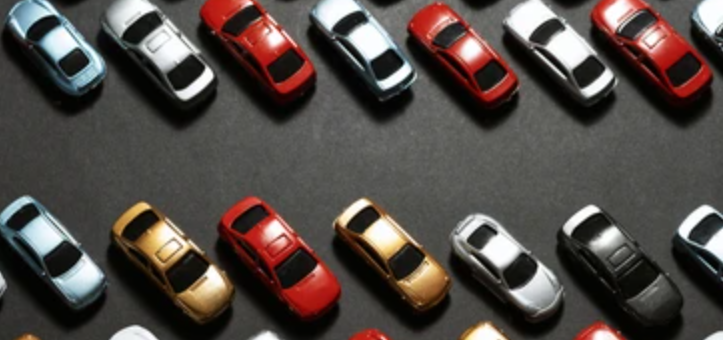
\includegraphics[scale=.23]{figs/cars.png} \\
\vspace{.5in}
\pause
{\tiny Solution: $2\times 3\times 4=24$ }


\end{frame}








\section{{\bf Ordered}  Arrangements {\bf with} Replacements }





\begin{frame}

\begin{itemize}
\qBrd[4.3in]{babyblue!30}{
\item[\sqBullet{babyblue}] Terminology:  \HLTY{\text{Order in Arrangements}} is\\
\begin{center}
 \HLTEQ[lime]{\text{Important}} or \HLTEQ[pink]{\text{ Not Important}}
 \end{center}
  }

\vspace{.2in}

\qBrd[4.3in]{blue!30}{
\item[\sqBullet{blue}] Terminology:  Arrangements\\
\begin{center} \HLTW{\text{With Replacement}} or  \HLTY{\text{Without Replacement}}  \end{center} }
\end{itemize}

\end{frame}


\begin{frame}\frametitle{Example}
Rearranging the letters of a word: ``EARTH"\\
Rearranging the letters of a word: ``TEN"     \\ 
Rearranging the letters of a word: ``SILENT"  \\
\vspace{1.5in}


$\Col{{\Row{\MCQ[2.1in]{
Order is Important 
} , \MCQ[2.1in]{
Order is NOT Important
}}},{\Row{\MCQ[2.1in]{ 
WITH Replacement
},\MCQ[2.1in]{
WITHOUT Replacement
}}}}$

\end{frame}



\begin{frame}\frametitle{Example}
How many 4 letter different `words' ({\tiny sequences of 4 letters}) can be constructed using the letters of   ``EARTH" ( {\tiny you may use same letters on multiple occasions })\\
\vspace{1.5in}


$\Col{{\Row{\MCQ[2.1in]{
Order is Important 
} , \MCQ[2.1in]{
Order is NOT Important
}}},{\Row{\MCQ[2.1in]{ 
WITH Replacement
},\MCQ[2.1in]{
WITHOUT Replacement
}}}}$

\end{frame}



\begin{frame}\frametitle{Example}
How many different 4 digit numbers can be constructed using the digits of the number ``12345"
\vspace{1.5in}


$\Col{{\Row{\MCQ[2.1in]{
Order is Important 
} , \MCQ[2.1in]{
Order is NOT Important
}}},{\Row{\MCQ[2.1in]{ 
WITH Replacement
},\MCQ[2.1in]{
WITHOUT Replacement
}}}}$

\end{frame}


\begin{frame}\frametitle{Example}
How many different 4 digit numbers can be constructed?
\vspace{1.5in}


$\Col{{\Row{\MCQ[2.1in]{
Order is Important 
} , \MCQ[2.1in]{
Order is NOT Important
}}},{\Row{\MCQ[2.1in]{ 
WITH Replacement
},\MCQ[2.1in]{
WITHOUT Replacement
}}}}$

\end{frame}








\TransitionFrame[bittersweet]{\Large {\bf Ordered}  Arrangements of {\bf distinct} objects {\bf with} Replacements   }


\begin{frame}{Ordered Arrangements of Distinct Objects  {\bf with} Replacements }
\begin{center}
\define{Ordered Arrangements with Replacement}{
Let $\HLTW{n, r}$ be positive  integers.  Number of different ways a sequence of $\HLTW{r}$ symbols can be created from $\HLTW{n}$ distinct symbols (when repetition of the symbols are allowed) is $\HLTEQ[yellow]{n^r}$. \\
\vspace{.1in}}
\vspace{-.2in}
\qBrd[4.3in]{amethyst!30}{ \tiny You may also view the procedure as the following: Number of different ways $r-$tuples (a vector with $r$ coordinates) can be constructed where elements of each coordinates are chosen arbitrary from a set containing $n$ distinct objects.  }\\
\vspace{1.2in}


\end{center}
\end{frame}



\begin{frame}
\vspace{-.2in}
\qBrd[4.6in]{babyblue!60}{ \Exmpl{babyblue!30}{} How many different numbers can be constructed using a 32 bits binary digits? 
} 
\vspace{-.25in}
\begin{center}
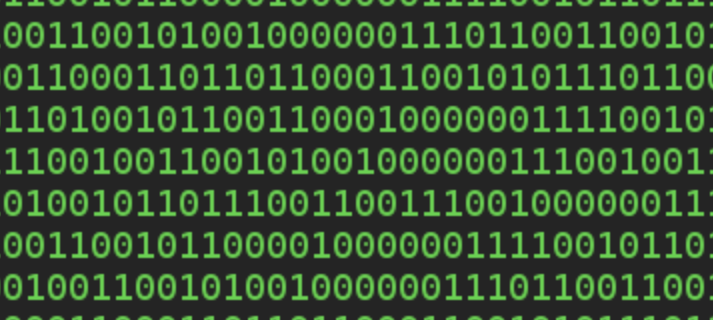
\includegraphics[scale=.4]{figs/bits.png} \\
\end{center}

\vspace{1.15in}
\pause
{\tiny Solution:  \HLT[yellow]{$2^{32}$}}

\end{frame}


\begin{frame}
	\frametitle{Example }
\qbx[4.5in]{cherryblossompink!50}{
\Exmpl{cherryblossompink}{} A typical lisence plate number in Abu-Dhabi consists of 5 digits.  How many different lisence plate numbers (excluding `00000') are possible ? 
}\\
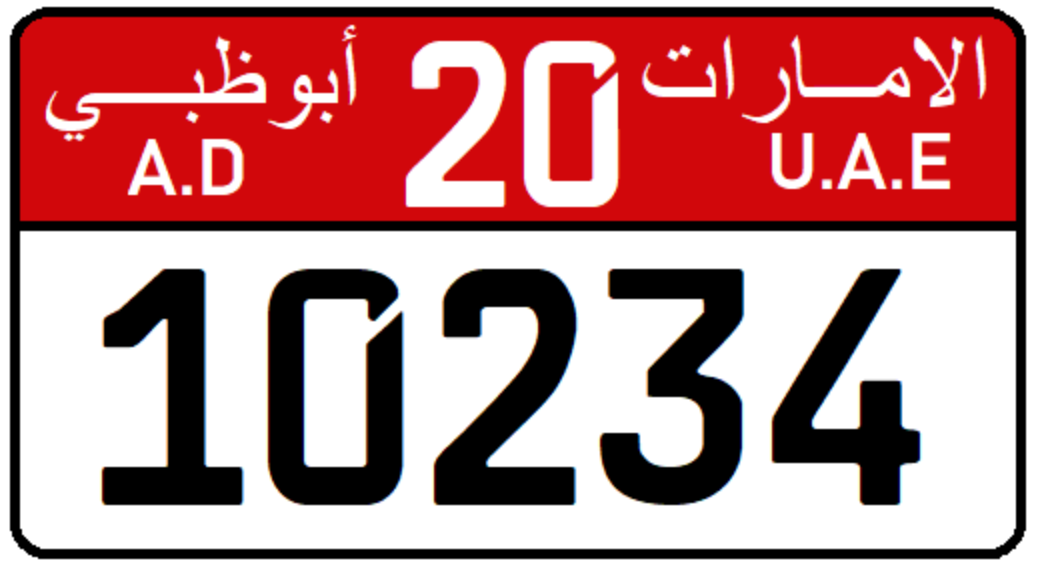
\includegraphics[scale=.2]{figs/L_Plate.png} \\
\vspace{1in}
\pause
{\tiny Solution: By the generalized version of the basic principle, the answer is $10^5-1=9999$}

\vspace{1in}
\end{frame}



\begin{frame}
\vspace{-.1in}
\qBrd[4.5in]{applegreen!30}{ \Exmpl{applegreen!50}{} From the numbers \{1, 2, \ldots ,44\}, a person
may pick any six for her ticket.  How many different groups of six numbers can be chosen from the forty-four {\bf if the repeated selection of the numbers is allowed while the same numbers selected in a different order is considered different sequence?
} }

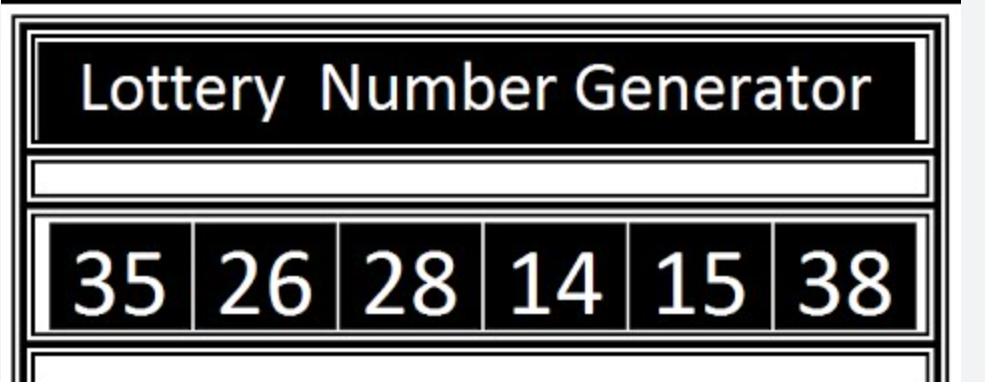
\includegraphics[scale=.25]{figs/lottery.png} \\
\vspace{.8in}
\pause
{\tiny Solution:  \HLT[yellow]{$44^6$}}

\end{frame}




\section{Permutations:{\small {\bf Ordered} Arrangements  of {\bf distinct} objects  {\bf Without} Replacements}    }


\TransitionFrame[bittersweet]{\Large Permutations:{\small {\bf Ordered} Arrangements {\bf distinct} objects {\bf Without} Replacements}    }

\begin{frame}\frametitle{Reminder: Factorial}


%\define{Factorial}{
%For a positive integer $n$, $n!$ (read $n$ factorial) is the product of
%all of the positive integers less than or equal to $n$. That is,
%$\HLTY{\HLTW{n!} = n \times  (n - 1) \times (n - 2) \times  \ldots  \times  3 \times  2 \times  1.}$
%Furthermore, we define $\HLTEQ[purple!30]{\HLTW{0!} = 1}$.}

\define{Factorial}{
Let $n$ be a {\bf non-negative integer,} then the {\bf factorial of n}, denoted as $\HLTY{n!}$ is defined to be
\begin{enumerate}
\item $\HLTEQ[purple!30]{\HLTW{0!} = 1}$,
\item $\HLTEQ[amethyst!40]{\HLTW{1!}=\HLTY{1}}$, 
\item $\HLTEQ[applegreen!40]{\HLTW{n!}= \HLTY{n\times(n-1)\times \cdots \times 1}}$ for $n\geq 2$
\end{enumerate} 
}

\vspace{.1in}
\pause
\qBrd[4.5in]{olive!30}{Example: $4!=4\times 3\times 2\times 1=24.$}
\qBrd[4.5in]{babyblue!30}{Example: $6!=6\times 5 \times 4\times 3\times 2\times 1=720.$}\\
\vspace{.05in}
\qBrd[4.5in]{amethyst!40}{\sqBullet{amethyst}Note that $\HLTW{n!}=n\times \{\HLTW{(n-1)!}\}$, for $n$ integer and  $n\geq 1$.}








\end{frame}



\begin{frame}
\vspace{-.1in}
\begin{center}
\define{Permutations (Ordered, without replacement)}{ Let $r$ be a positive integer such that $r\leq n$.  An ordered arrangement of $r$ distinct objects is called a permutation.  The number of ways of ordering $n$ distinct objects taken $r$  at a time will be designated by the symbol $^nP_r$. \vspace{-.18in}   Note that  $$\HLTEQ[applegreen!50]{ \HLTW{\displaystyle  ^nP_r}=  \HLTEQ[white]{ \displaystyle n(n - 1)(n- 2)(n - r + 1) }= \HLTW{ \displaystyle \frac{n!}{(n - r )!}  }   }.$$
\vspace{.2in}
}
\vspace{-.3in}
\qBrd[4.3in]{teal!40}{This is also the different ways $r$ different objects can be chosen from n different objects  when the order of the choice is  important.  However, there is no repetition in the choices of $r$ objects. }
\end{center}
\qbx[4.5in]{ceil!50}{\sqBullet{ceil}The number of possible permutations of n distinct objects is
given by: $\HLTW{\displaystyle ^nP_n= n! =n\times (n-1) \times \cdots \times 2\times 1}$. }

\vspace{1in}
\end{frame}





\begin{frame}
\vspace{-.2in}
\qBrd[4.5in]{iceberg!30}{ \Exmpl{iceberg!70}{} From the numbers \{1, 2, \ldots ,44\}, a person
may pick any six for her ticket.  How many different groups of six numbers can be chosen from the forty-four {\bf if the repeated selection of the numbers are {\it NOT allowed}  while the order at which the numbers are selected is important.}
}\\
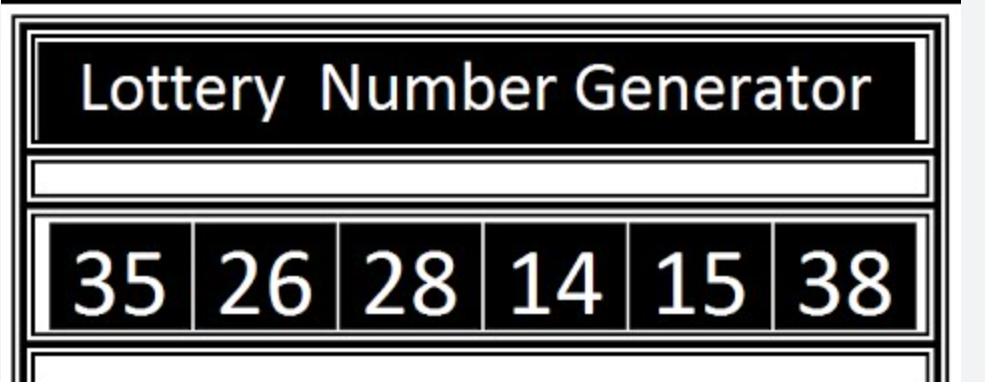
\includegraphics[scale=.25]{figs/lottery.png} \\
\pause 
\vspace{.8in}
{\tiny
Solution: \HLT[yellow]{$ ^{44}P_{6}= 44\time 43 \times 42\times 41\times 40 \times 39 $}}
\end{frame}




\begin{frame}
\qbx[4.5in]{bluebell!40}{\Exmpl{bluebell}{}
How many different batting orders are possible for a
baseball team consisting of 9 players?}\\
\vspace{2.5in}
\pause
{\tiny
 Solution: There are $9! = 362880$ possible batting orders. }
\end{frame}


\begin{frame}
\qbx[4.5in]{cambridgeblue!50}{\Exmpl{cambridgeblue}{}
How many different words can you make with the letters
\HLTW{\text{"CAN"}}?}\\
\vspace{2.5in}
\pause
{\tiny
 Solution:  $3! = 6$ }
\end{frame}




\begin{frame}
\vspace{-.1in}
\qbx[4.5in]{carnationpink!50}{\Exmpl{carnationpink}{}
A class in probability theory consists of 6 men and 4
women. An examination is given, and the students are ranked
according to their performance. Assume that no two students
obtain the same score.
\begin{enumerate}[(a)]
\item How many different rankings are possible?
\item  If the men are ranked just among themselves and the women
just among themselves, how many different rankings are possible?
\end{enumerate}}\\
\vspace{.7in}
\pause
{\tiny
 Solution:
 \begin{enumerate}[(a)]
 \item  Because each ranking corresponds to a particular
ordered arrangement of the 10 people, the answer to this part is
$10! = 3,628,800$.
\item  Since there are 6! possible rankings of the men among
themselves and 4! possible rankings of the women among
themselves, it follows from the basic principle that there are
$(6!)(4!) = (720)(24) = 17280$ possible rankings in this case.
\end{enumerate}  
}
\end{frame}







\section{Combinations: {\small Arrangements of {\bf distinct} objects {\bf without replacement} when {\bf order is not important}}   }



\TransitionFrame[bittersweet]{\Large Combinations: {\small Arrangements of {\bf distinct} objects {\bf without replacement} when {\bf order is not important}}  }




\begin{frame}{Combinations (Un-ordered, without replacement)}
\begin{center}
\vspace{-.1in}
\define{Combinations}{ The number of combinations of $n$ objects taken $r$ at a time is the number of subsets, each of size $r$ , that can be formed from the $n$ objects. 
This number, denoted by ${n\choose r}$ ( {\tiny or $^nC_r$)}, is given as \vspace{-.1in} $$\HLTEQ[babyblue!70]{\HLTW{ \displaystyle {n \choose r }}= \HLTW{ \displaystyle\frac{n!}{r! (n-r)!}}}$$
}
\vspace{-.2in}
\qBrd[4.1in]{amethyst!40}{
This is also the different ways $r$ different objects can be chosen from n different objects  when the order of the choice is not important. However, there is no repetition in the choices of $r$ objects. }
\end{center}
\vspace{.7in}


\end{frame}


\begin{frame}
\vspace{-.2in}
\qbx[4.6in]{amethyst!40}{\Exmpl{amethyst}{}
\small A motherboard has 8 slots, where we want to place 4
{\bf identical} cards.  How many unique possible way one can insert the 4 cards?}\\
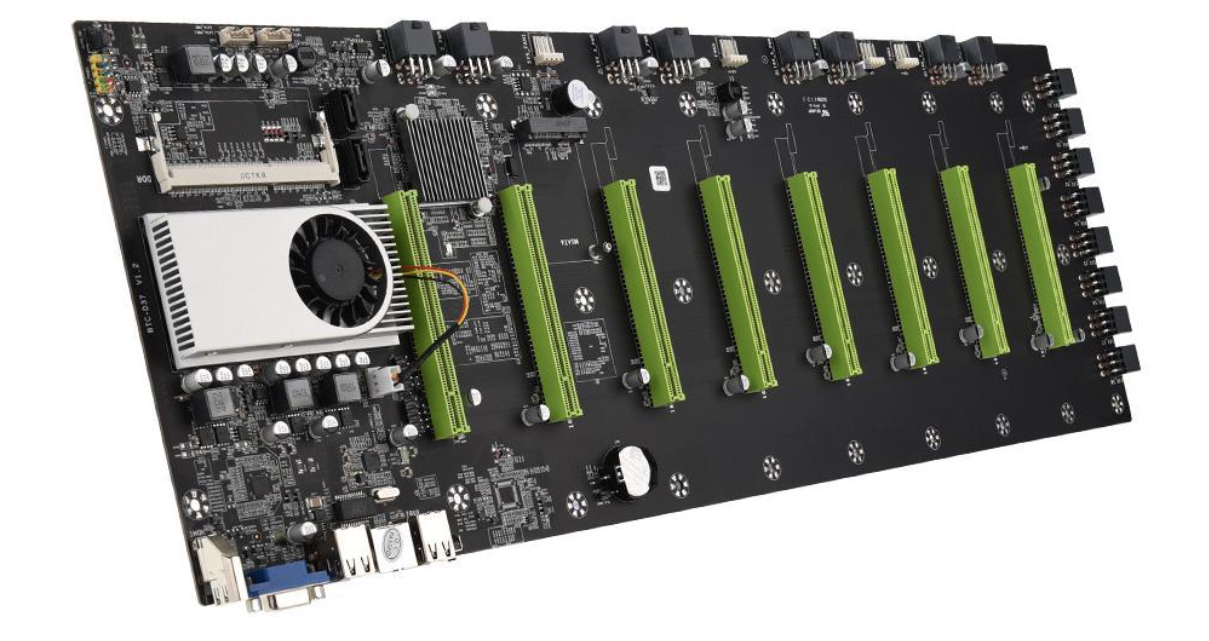
\includegraphics[scale=.25]{figs/motherboard.png}
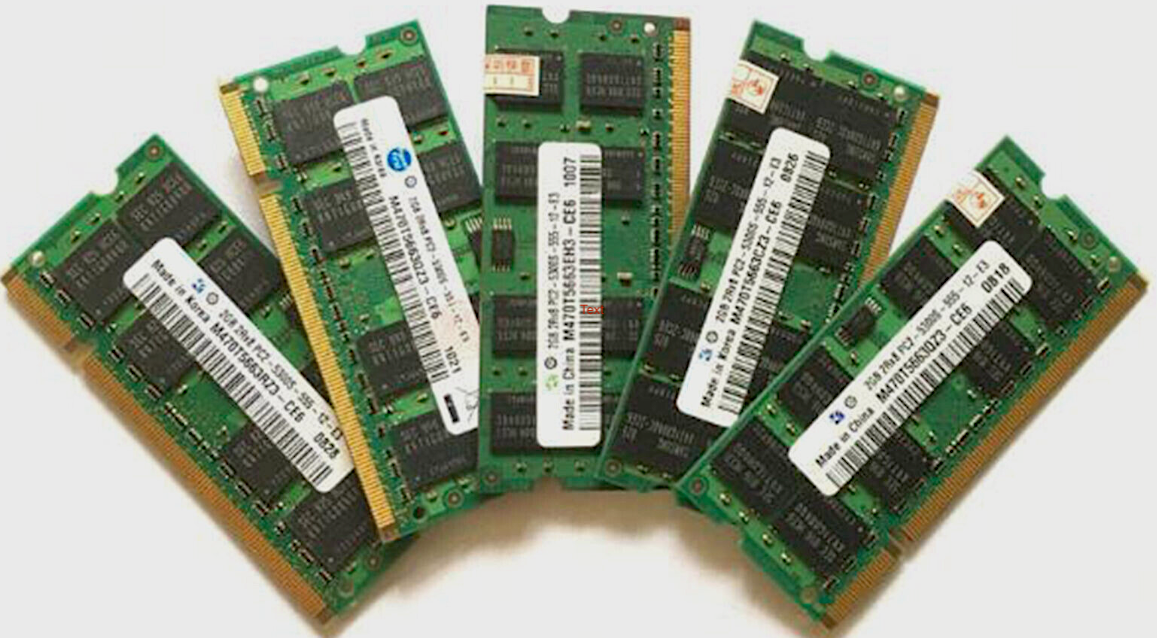
\includegraphics[scale=.2]{figs/slotCard5.png}\\
\pause
\vspace{1in}
 \HLT[yellow]{ \tiny Solution ${8 \choose 4 }= \frac{8!}{(8-4)! (4!)}$}  
\end{frame}




\begin{frame}
\vspace{-.2in}
\qBrd[4.5in]{iceberg!30}{ \Exmpl{iceberg!70}{} From the numbers \{1, 2, \ldots ,44\}, a person
may pick any six for her ticket.  How many different groups of six numbers can be chosen from the forty-four {\bf if the repeated selection of the numbers are {\it NOT allowed}  and the order at which the numbers are selected is  NOT important.}
}\\
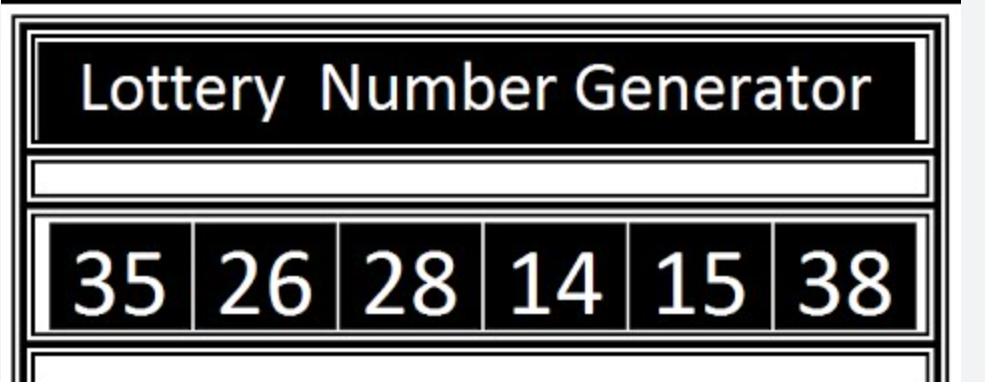
\includegraphics[scale=.25]{figs/lottery.png} \\
\pause 
\vspace{.8in}
{\tiny
Solution: \HLT[yellow]{${ {44}\choose 6}= \frac{44\time 43 \times 42\times 41\times 40 \times 39}{6\times 5\times 4\times 3\times 2\times 1} $}}
\end{frame}


\begin{frame}
\qbx[4.5in]{applegreen!40}{\Exmpl{applegreen}{}
From a group of 5 women and 7 men, how many
different committees consisting of 2 women and 3 men can be
formed? What if 2 of the men are feuding and refuse to serve on
the committee together? }\\
\vspace{1.5in}
\pause
 {\tiny Solution: ${5 \choose 2}\times {7 \choose 3}= 350$\\
 Now a total of ${2 \choose 2}\times {5 \choose 1}= 5 $ out of ${7 \choose 3}=35$ possible groups of 3
men contain both of the feuding men, it follows that there are 35 -5 = 30 groups that do not contain
both of the feuding men. Then, the possible number of committees becomes $30 \times 10 =300$
 }  
\end{frame}

\begin{frame}
\define{Multinomial Probability}{
The number of ways of partitioning $n$ distinct objects into $k$ distinct groups
containing $n_1$, $n_2$, . . . , $n_k$ objects, respectively, where each object appears in exactly one group and $\sum_{i=1}^{k}n_i=n$, is  
 $$\HLTEQ[yellow]{\large \displaystyle {n\choose {n_1, n_2, \ldots , n_k}}:= \frac{n!}{(n_1!)(n_2!)\ldots (n_k!)}}$$
}
\begin{center}
\qBrd[4.5in]{amber!40}{The above procedure is also utilized to determine the number of permutations of a set
of n objects when certain of the objects are indistinguishable
from each other.}
\end{center}
\end{frame}


\begin{frame}
\qbx[4.5in]{teal!40}{\Exmpl{teal}{}
How many different `words' ({\tiny it many not be a meaningful word though}) can you make with the letters of the word
\HLTW{\text{"PEPPER"}}?}\\
\vspace{2.5in}
\pause
{\tiny
 Solution:  $\frac{6!}{(3!)(2!)(1!)}$ }
\end{frame}




%\section{Arrangements {\bf With Replacement} When {\bf Order is Not Important} }
%
%\TransitionFrame[bittersweet]{ Arrangements {\bf With Replacement} When {\bf Order is Not Important}  }


\section{Arrangements of {\bf identical} Objects in Multiple Groups}
\TransitionFrame[bittersweet]{ Arrangements of {\bf identical} objects in Multiple Groups ({\tiny without replacement and order of objects in each selected group is not important. }) }

\begin{frame}{Unordered Arrangements of Identical Objects}
\begin{center}
\define{Unordered Arrangements of Identical Objects}{
Number of ways $n$ indistinguishable objects can be organized into r different groups is $$\HLTW{\displaystyle \frac{(n+r-1)!}{n! (r-1)!}={{n+r-1} \choose {n}}}.$$
}
\vspace{-.2in}
\qBrd[4.1in]{guppiegreen!30}{The processes can viewed as: How many different ways $n$ identical  balls can be placed in $r$ different urns.  Ordering of the groups are not important.  }\\
%
%\qBox{\Qn: How many different solutions  $(X_1, X_2, \ldots, X_r)$ are there satisfying the equation $X_1+X_2+\ldots + X_r=n$ where we assume $X_i $ to be non-negative integer for all $i=1, \ldots, r$.}
\vspace{.1in}
\qBrd[4in]{amethyst!40}{\sqBullet{amethyst} It is also referred to as the occupancy problem }

\vspace{.1in}
\qBrd[4in]{amber!40}{ \sqBullet{amber}In the textbook it is referred to as: ``THE NUMBER OF INTEGER SOLUTIONS OF EQUATIONS''}
\end{center}


\end{frame}






\begin{frame}
\qbx[4.5in]{apricot!40}{\Exmpl{apricot}{}
How many different solutions are there for the following equation?
$\HLTW{x_1+x_2+x_3+x_4+x_5=10}$ if $x_1, x_2, x_3, x_4,x_5$ are all non-negative integers?
}\\
\vspace{2in}
\pause
{\tiny
 Solution:  ${14 \choose 4}= 1001$  }
\end{frame}



%
%\begin{frame}
%\qBrd[4.5in]{iceberg!30}{ \Exmpl{iceberg!70}{} From the numbers \{1, 2, \ldots ,44\}, a person
%may pick any six for her ticket.  How many different groups of six numbers can be chosen from the forty-four {\bf if the repeated selection of the numbers are allowed while the order at which the numbers are selected is not important.}
%}\\
%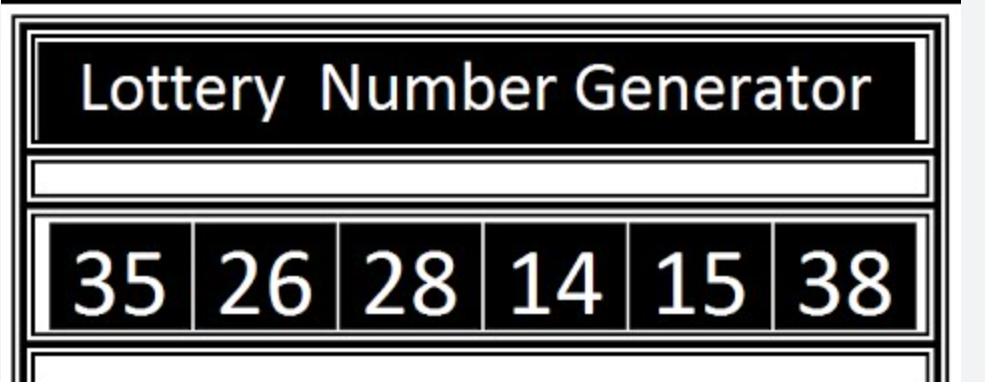
\includegraphics[scale=.25]{figs/lottery.png} \\
%\pause 
%\vspace{.8in}
%{\tiny
%Solution: \HLT[yellow]{$\frac{(6+44-1)!}{(43!) (6!)}={{49} \choose {43}}$}}
%\end{frame}



\section{Miscellaneous Problems On Counting}

\TransitionFrame[amethyst]{ Miscellaneous Problems On Counting }


\begin{frame}
\qbx[4.5in]{brightube!40}{\Exmpl{brightube}{}
Consider 6 tosses of a coin.  For example two typical sequences of outcomes that are considered different is  `HTTTTT', and `THTTTT'.
\begin{enumerate}[a).]
\item What is the total number of different outcomes from the experiment?
\item  How many different ways there can be exactly 2 heads?
\end{enumerate} 
}\\
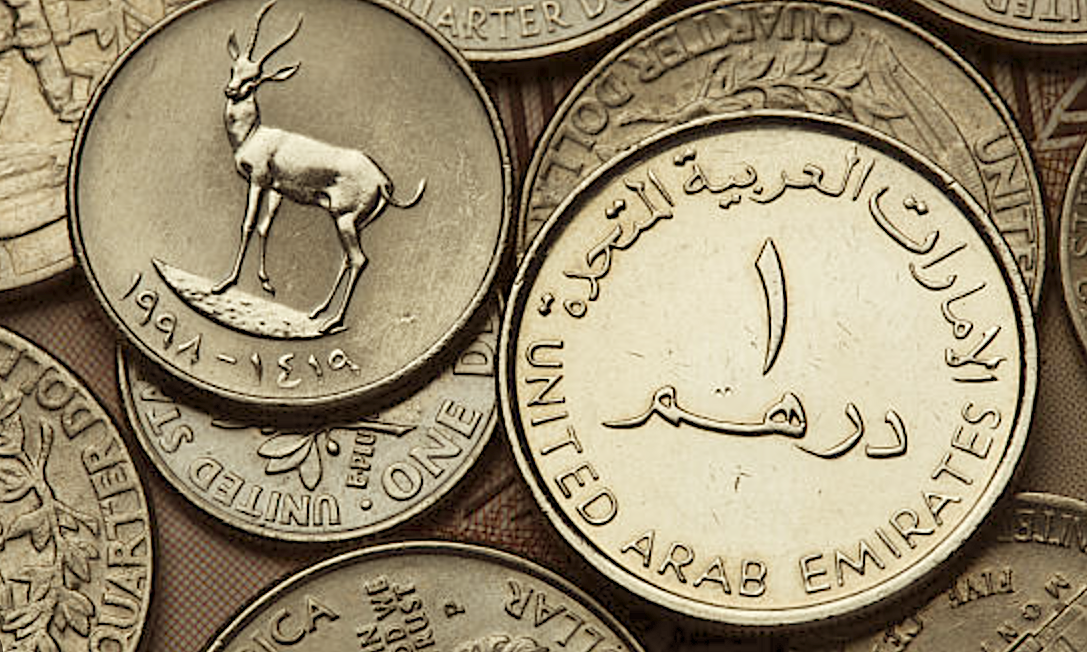
\includegraphics[scale=.2]{figs/coin.png} \\
\vspace{.5in}
\pause
{\tiny
 Solution: a)  ${2^6}= 64$,  b) ${6 \choose 2}$  }
\end{frame}




\begin{frame}
\qBrd[4.5in]{purple!30}{ \Exmpl{purple!50}{} If a dice is thrown 4 times and all the the 4 numbers (4-tuple) that appear are recorded.  
\begin{enumerate}[a).]
\qBrd[4in]{camel!40}{ \item What is the total number of  distinct possibilities of the 4 numbers (distinct 4-tuples) that can occur?}
\qBrd[4in]{amber!40}{ \item In how many such 4-tuples, there will be exactly two 5s?}
\qBrd[4in]{olive!40}{ \item In how many such 4-tuples, there will be no 6?}
\qBrd[4in]{babyblue!40}{ \item In how many such 4-tuples, there will be at least one  6?}
\end{enumerate}
\vspace{.05in}
} 

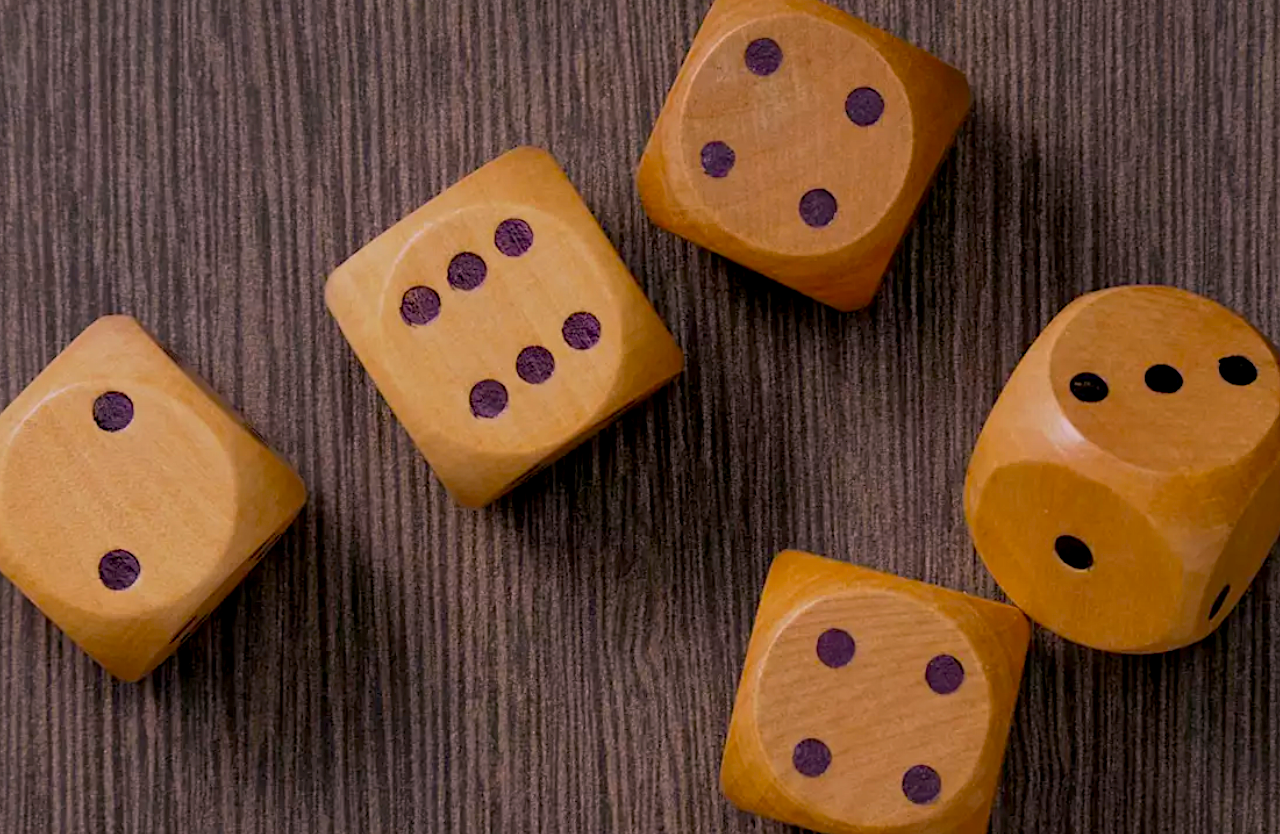
\includegraphics[scale=.15]{figs/dice.png} \\
\vspace{.3in}
\pause
{\tiny Solution: 
a)$ \HLTY{6^4}$, b) $\HLTY{{4\choose 2} 5^2}$, c) $\HLTY{5^4}$ d) $\HLTY{6^4-5^4}$
}

\end{frame}




\begin{frame}
\qbx[4.5in]{amber(sae/ece)!40}{\Exmpl{amber(sae/ece)}{} {\tiny Passwords are a context where it is interesting to count and compare the total number of possible ways when the length is relatively small and as restrictions are introduced or relaxed. } \\
A typical ATM pin consists of 4 digits.  
\begin{enumerate}
\item How many different (unique) 4 digit passwords can be constructed if digits are restricted to be only numeric? 
\item How many different (unique) 4 digit passwords can be constructed if the First digit must be an English alphabet while rest are numeric? 
\item How many different (unique) 4 digit passwords can be constructed if the digits can either be any number or English alphabet? 
\end{enumerate}  }\\
\includegraphics[scale=.25]{figs/ATMPIN.png} \\
\pause 
\vspace{1.5in}
%\pause
%{\tiny
 %Solution:  $\frac{10!}{(4!)(3!)(2!)(1!)}$ }
\end{frame}








\begin{frame}
\qbx[4.5in]{rose!40}{\Exmpl{rose!70}{} \\
What is the number of  unique permutations for the letters in the word `BANANA'? }\\
\vspace{1.5in}
%\pause
%{\tiny
 %Solution:  $\frac{10!}{(4!)(3!)(2!)(1!)}$ }
 \vspace{2in}
\end{frame}




\begin{frame}
\qbx[4.5in]{olive!40}{\Exmpl{olive}{}
Consider a Set $A=\{a_1, a_2, a_3 , a_4\}$ containnig $4$ elements.  
\begin{enumerate}[a).]
\item What is the total number of different subsets of the set $A$ that has exactly $2$ elements in it?
\item What is the total number of different subsets of the set $A$?
\item What is the total number of different non empty proper subsets of the set $A$?
\end{enumerate} 
}\\
\vspace{1in}
\pause
{\tiny
 Solution: a) ${4 \choose 2}$ b)  ${2^4}= 16$,  c) $2^4-2=14$ }
 \vspace{.11in}
\end{frame}



\begin{frame}
\qbx[4.5in]{applegreen!40}{\Exmpl{applegreen}{}
Ms. Jones has 10 books that she is going to put on
her bookshelf. Of these, 4 are mathematics books, 3 are chemistry
books, 2 are history books, and 1 is a language book. Ms. Jones
wants to arrange her books so that all the books dealing with the
same subject are together on the shelf. How many different
arrangements are possible?}\\
\vspace{1.5in}
\pause
{\tiny
 Solution: There are $4! 3! 2! 1!$ arrangements such that the
mathematics books are first in line, then the chemistry books, then
the history books, and then the language book. Similarly, for each
possible ordering of the subjects, there are $4! 3! 2! 1!$ possible
arrangements. Hence, as there are $4!$ possible orderings of the
subjects, the desired answer is $4! (4! 3! 2! 1!) = 6912$. }
\end{frame}


\begin{frame}
\qbx[4.5in]{teal!40}{\Exmpl{teal}{}
One of the sections in the class STAT230 has 8 students.  Assume the birthday of a student can be any one of days out of 365 days in a year.  We say that the two students share a same birth day if they are born on the same day and same month {\tiny ( for example two students are born on $10^{\text{th}}$ January).}  Answer the follwoing questions. 
\begin{enumerate}[a).]
\item What is the total number of different possibilities for the birthday of the 8 students?
\item How many different possibilities are there such that  exactly two students have the same birthday?
\item How many different possibilities are there if exactly four of students have the same birthday?
\item How many different possibilities are there so that all the birthdays are on different day of the year. 
\end{enumerate} 
}\\
%\vspace{.1in}
\pause
{\tiny
 Solution: a)$ 365^8$ b)  $365\times  {8 \choose 2} 364\times \cdots \times 359$ c)  $365\times {8 \choose 4} \times 364\times 363\times 362 \times 361$  c) $^{365}P_{8}$ }
 \vspace{.11in}
\end{frame}




%
%
%\begin{frame}
%\vspace{-.5in}
%\qbx[4.5in]{amethyst!40}{\Exmpl{amethyst}{}
%A chess tournament has 10 competitors, of which 4
%are Russian, 3 are from the United States, 2 are from Great Britain,
%and 1 is from Brazil. If the tournament result lists just the
%nationalities of the players in the order in which they placed, how
%many outcomes are possible?}\\
%\vspace{1.1in}
%\pause
%{\tiny
% Solution:  $\frac{10!}{(4!)(3!)(2!)(1!)}$ }
%\end{frame}
%





\begin{frame}
	\frametitle{Example }
\qbx[4.5in]{cherryblossompink!40}{
\Exmpl{cherryblossompink}{} How many different 7-place license plates are possible if the first 3 places are to be occupied by letters and the final 4 by numbers?
}\\
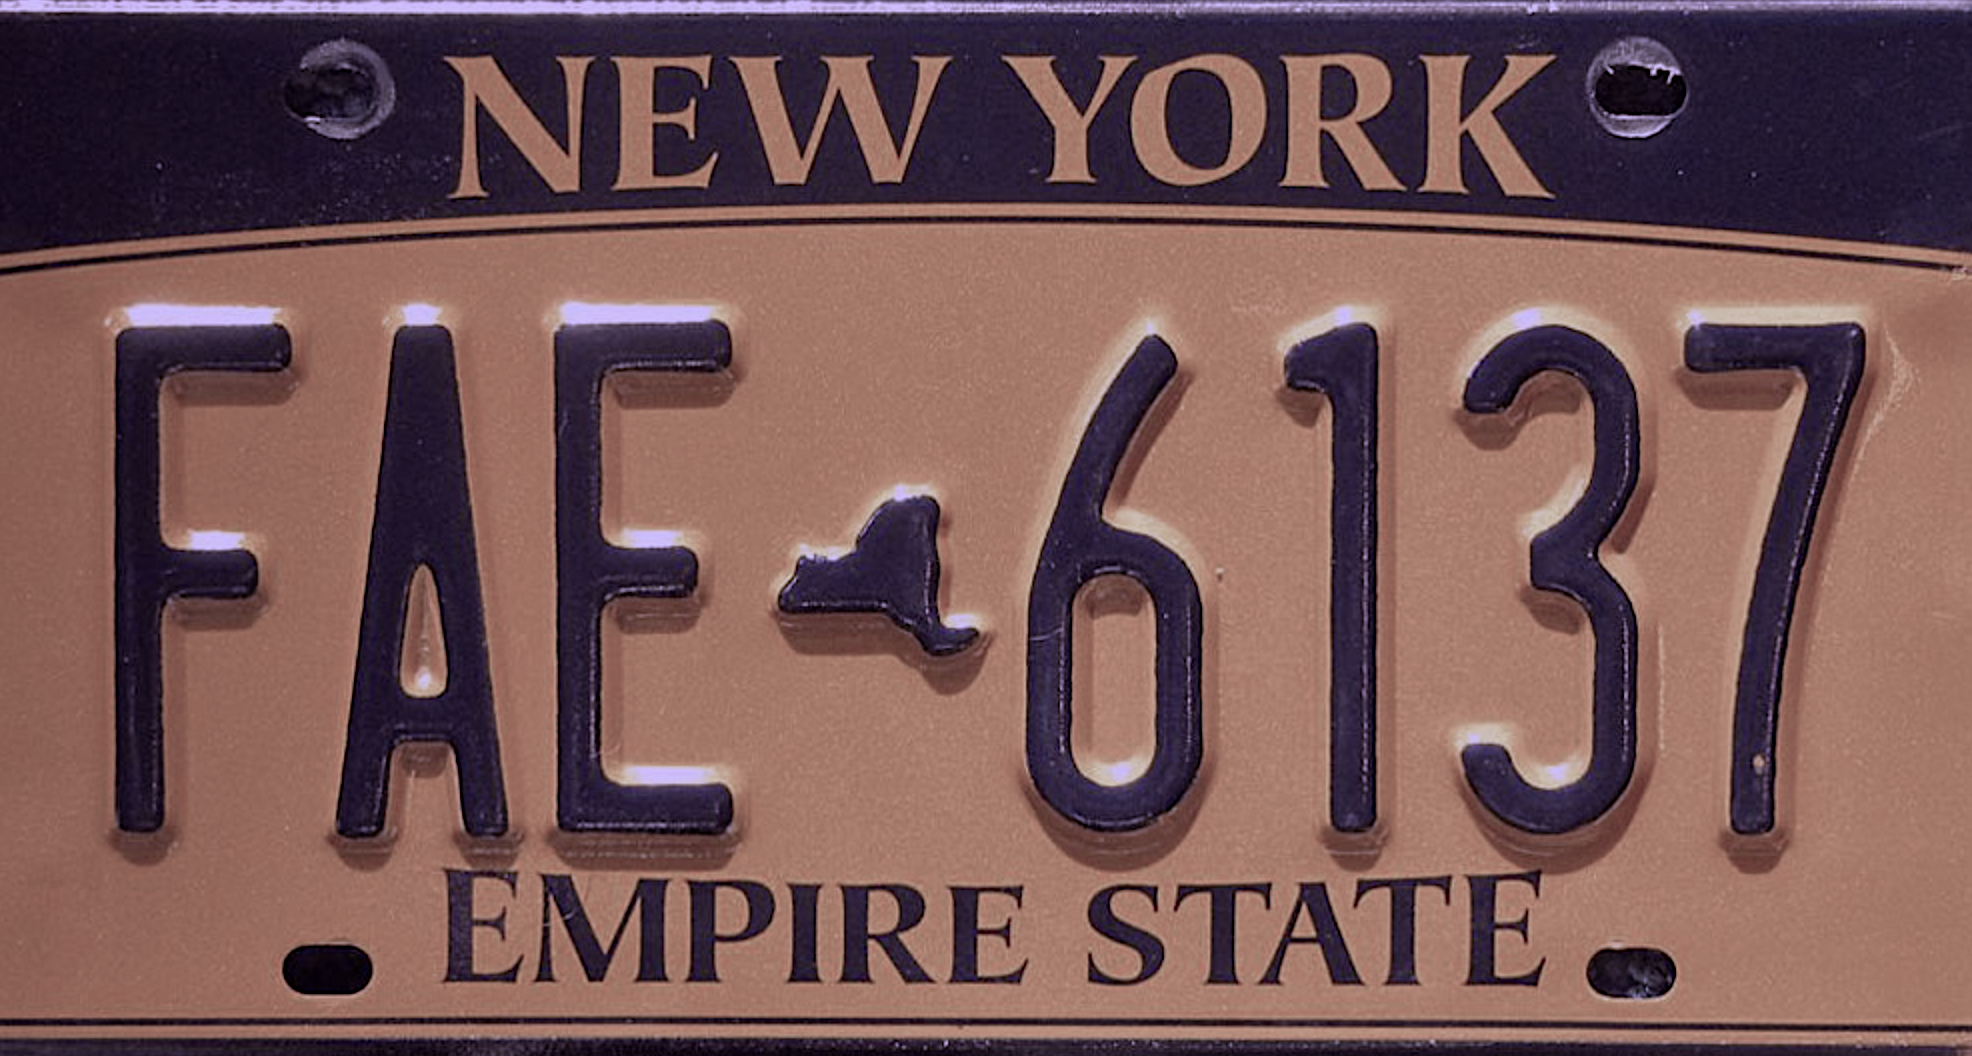
\includegraphics[scale=.1]{figs/NewYork_Plate.png} \\
\pause 
\vspace{.9in}
\pause
{\tiny Solution: By the generalized version of the basic principle, the answer is $26\times 26\times 26 \times 10\times 10\times 10\times 10 = 175, 760,000.$}

\vspace{1in}
\end{frame}






\begin{frame}
%\vspace{-.5in}
\qbx[4.6in]{teal!40}{\Exmpl{teal}{}
How many different signals, each consisting of 9 flags hung in a line, can be made from a set of 4 white  flags, 3 red  flags, and 2 blue  flags if all  flags of the same color are identical?}\\
\begin{center}

\includegraphics[scale=.23]{figs/9Flags.png}
\end{center}
\vspace{1.2in}
\pause
{\tiny
 Solution:  $\frac{9!}{(4!)(3!)(2!)}$ }
\end{frame}



\begin{frame}
%\vspace{-.5in}
\qbx[4.6in]{babyblue!40}{\Exmpl{babyblue}{}
How many different signals, each consisting of 9 flags hung in a line, can be made from a set of 4 white  flags, 3 red  flags, and 2 blue  flags if all  flags of the same color but can be uniquely identified by their number that is written on them?}\\
\begin{center}
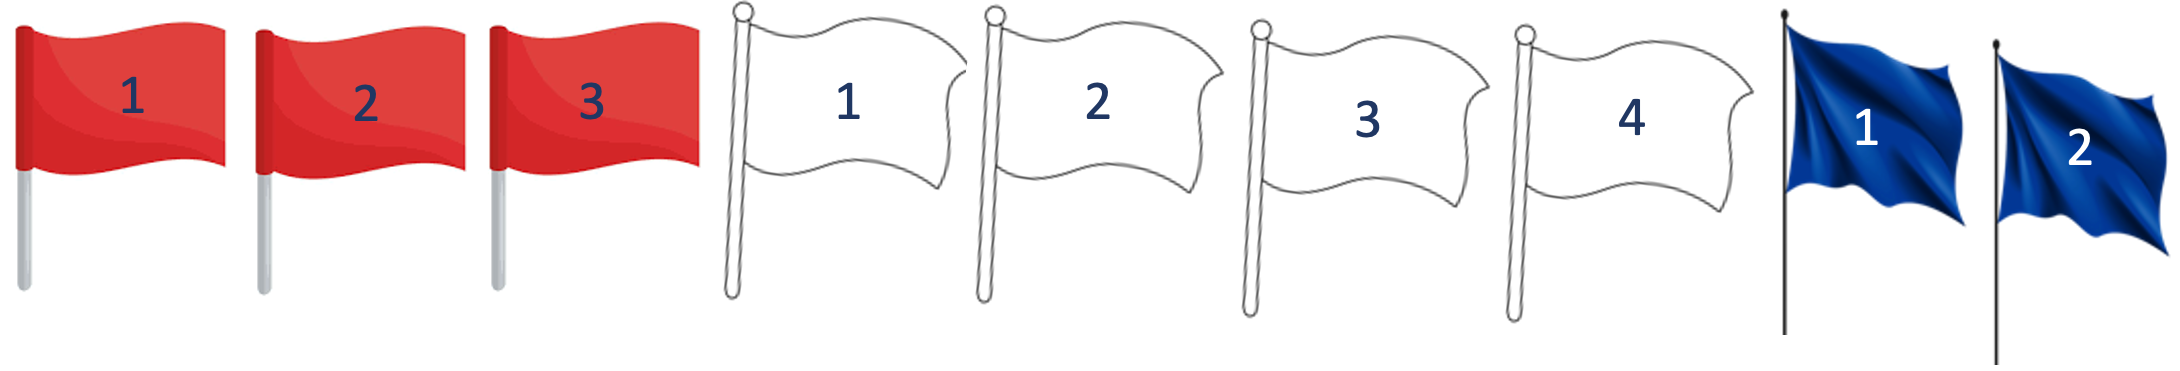
\includegraphics[scale=.23]{figs/9FlagNumber.png}
\end{center}
\vspace{1.2in}
\pause
{\tiny
 Solution:  $9!$ }
\end{frame}




\begin{frame}
\qbx[4.5in]{antiquefuchsia!40}{\Exmpl{antiquefuchsia}{}
Consider a group of 20 people. If everyone shakes
hands with everyone else, how many handshakes
take place?}\\

\includegraphics[scale=.2]{figs/HandShake.png} 

\vspace{1.5in}
\pause
{\tiny
 Solution:  ${20 \choose 2}$ }
\end{frame}





\begin{frame}
\qbx[4.5in]{apricot!40}{\Exmpl{apricot}{}
An investor has 20 thousand dollars to invest among 4 possible investments.  Each investment must be in units of a thousand dollars. If the total 20 thousand is to be invested, 
\begin{enumerate}
\item how many different investment strategies are possible?
\item  how many different investment strategies are possible  if not all the money need be invested?
\end{enumerate}    
}\\
\vspace{1.5in}
\pause
{\tiny
 Solution: a) ${23 \choose 3}= 1771$ , b)  ${24 \choose 4}= 10,626$ }
\end{frame}



\begin{frame}
\begin{minipage}{.6\textwidth} %
\vspace{-.25in}
\qBrd[3.1in]{airforceblue!60}{\;
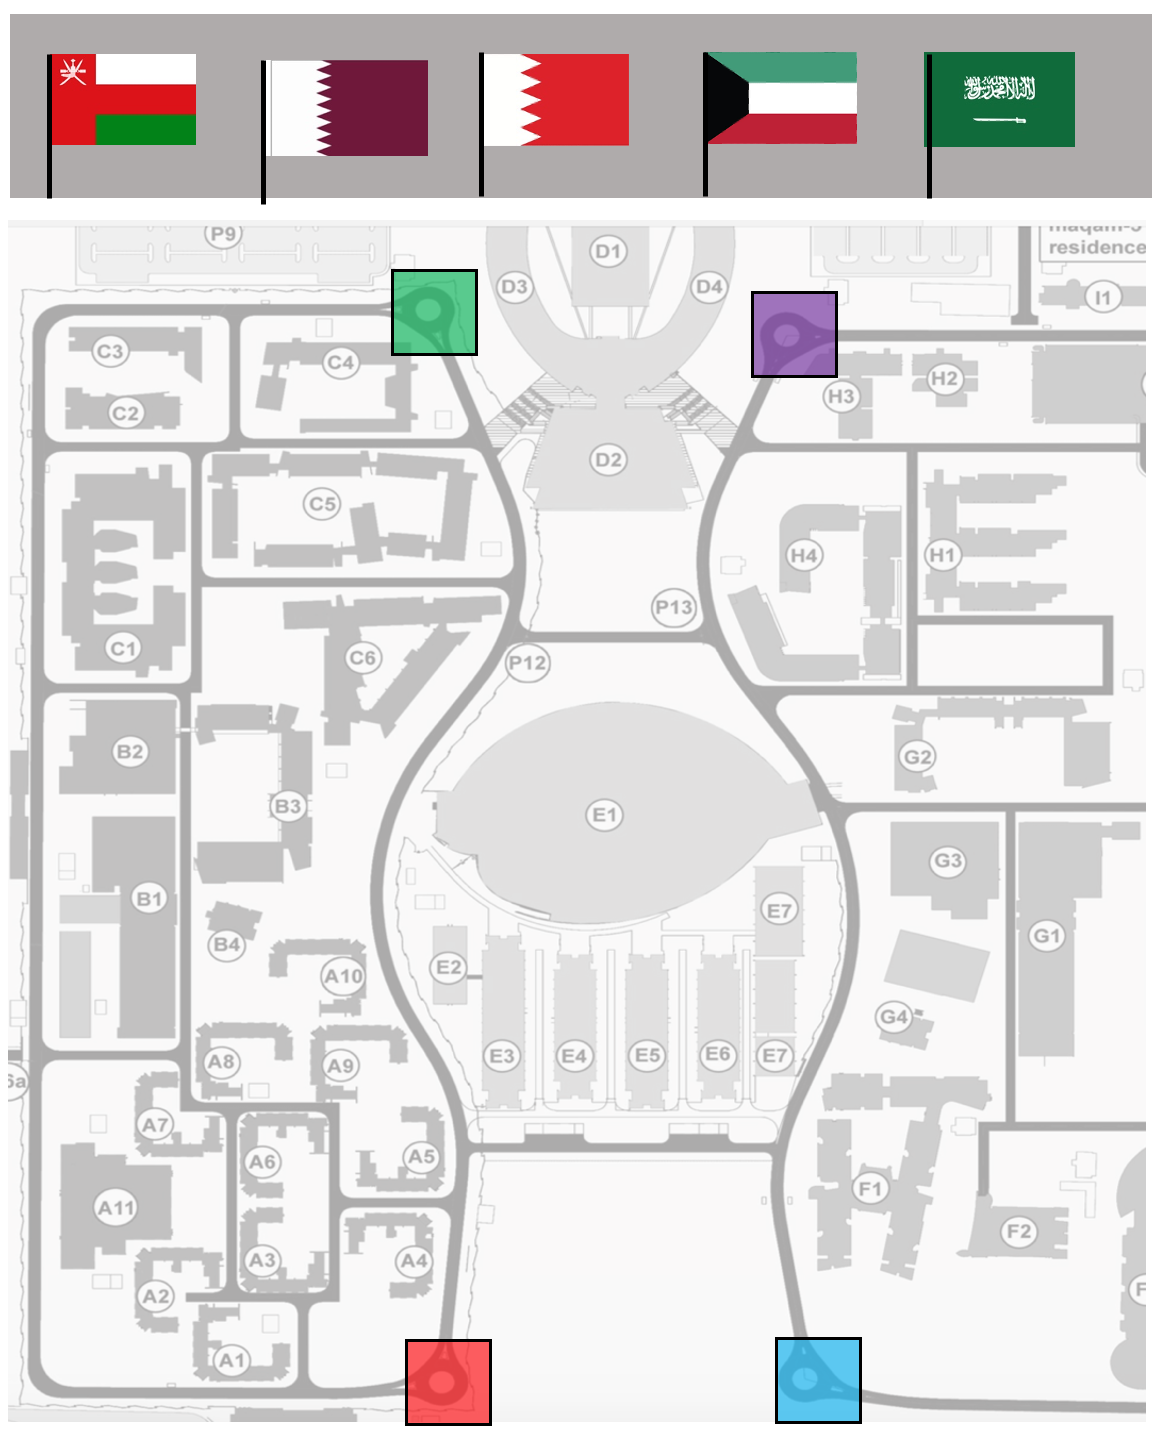
\includegraphics[scale=.33]{figs/UAEU_FLAG_GCC.png}
}
\end{minipage}
\;\;\;\;
\begin{minipage}{.32\textwidth} %
\qbx[1.45in]{amethyst!40}{\Exmpl{amethyst}{}
\small How many different ways one can arrange  5 distinct flags in  4 different locations? Assume that each of the locations are considered to have exactly one flag to put.  
}
\vspace{1.95in}
\end{minipage} %



{\tiny
 Solution:  }
\end{frame}





\begin{frame}
\begin{minipage}{.6\textwidth} %
\vspace{-.2in}
\qBrd[3.1in]{airforceblue!60}{\;
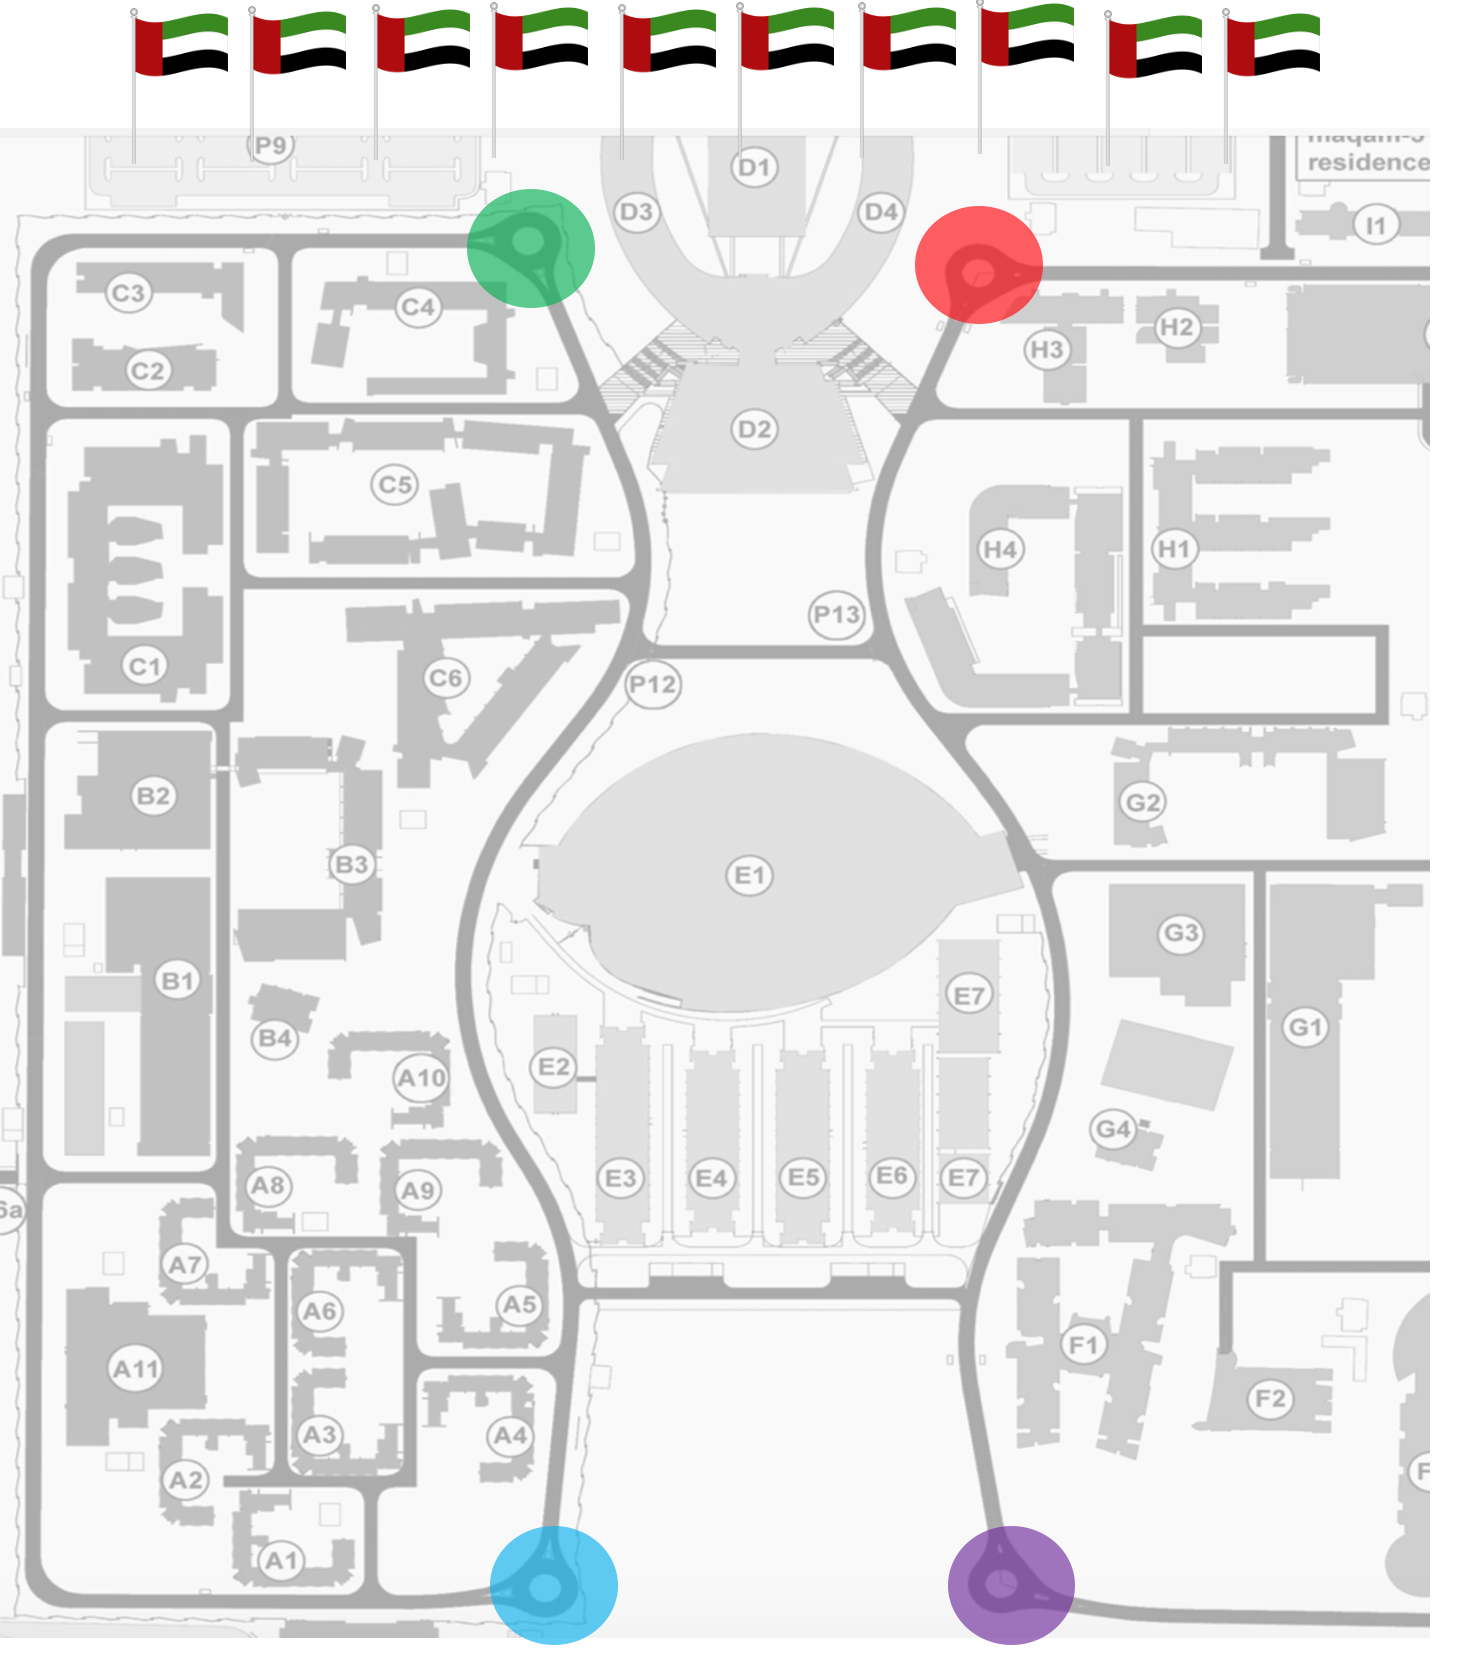
\includegraphics[scale=.3]{figs/UAEU_FLAG_UAE.png}
}
\end{minipage}
\;\;\;\;
\begin{minipage}{.32\textwidth} %
\qbx[1.45in]{lime!40}{\Exmpl{lime}{}
\small How many different ways one can arrange  10 identical flags in  4 different locations? Assume that,  a location may have zero, one or  more than one flags.
}
\vspace{1.95in}
\end{minipage} %



{\tiny
 Solution:  }
\end{frame}





\begin{frame}
\qbx[4.5in]{babyblue!40}{\Exmpl{babyblue}{}
A police department in a small city consists of 10
officers. If the department policy is to have 5 of the officers
patrolling the streets, 2 of the officers working full time at the
station, and 3 of the officers on reserve at the station, how many
different divisions of the 10 officers into the 3 groups are possible? }\\
\vspace{2in}
\pause
{\tiny
 Solution:  $\frac{10!}{(5!)(2!)(3!)}= 2520$ }
\end{frame}




\begin{frame}
\qbx[4.5in]{green!40}{\Exmpl{green}{}
Ten children are to be divided into an A team and a
B team of 5 each. The A team will play in one league and the B
team in another. How many different divisions are possible? }\\
\vspace{2.5in}
\pause
{\tiny
 Solution:  ${10 \choose 5}=\frac{10!}{(5!)(5!)}= 252$ }
\end{frame}




\TransitionFrame[bittersweet]{\Large Binomial and Multinomial Coefficient  }







\TransitionFrame[antiquefuchsia]{\Large Questions?  }
 
 
\end{document}
